%
% Draft  document crimpmeas.tex
% Notes on crimp formation in wool staples
%
 
\documentclass[titlepage,10pt]{article}  % Latex2e
\usepackage{graphicx,lscape,subfigure}
\usepackage{bm}
\usepackage{textcomp}
 

\title{ Measuring the wavelength and amplitude of crimp in Merino staples}
\author{Jim Watts and Neville Jackson}
\date{18 Sep 2016} 

 
\begin{document} 
 
\maketitle      
\tableofcontents

\clearpage
\section{Introduction} 
 In a study of  crimp formation in Merino wool staples ( Jackson and Watts(2016)~\cite{jack:16}) the authors have developed a mathematical model for staple crimp formation which allows the calculation of intrinsic fibre curvature, mean fibre length, and fibre length to staple length ratio. The calculation requires measurements of the crimp wavelength and amplitude.

This document deals with our efforts to devise a reasonable measurement technique for crimp wavelength and amplitude. This proved to be much more difficult than anticipated. Three different measuring techniques were tried. Their comparative evaluation required some extensive analyses, and these are reported here, rather than as part of the Jackson and Watts(2016)~\cite{jack:16} document.

\section{The sheep studied and measurements made}
 The 22 sheep studied in Jackson and Watts(2016)~\cite{jack:16} were measured for crimp frequency, crimp wavelength, and crimp amplitude.  These sheep were classified for crimp type into three groups, {\em unfolded}, {\em stretched}, and {\em unaligned}. Both the {\em stretched}, and {\em unaligned} groups were a stretched helix crimp type, with the latter having a less well defined crimp with many fibres out of phase. Crimp frequency was measured on staples using a ruler graduated in millimetres. Crimp wavelength and amplitude were measured using three techniques.
\begin{description}
\item[single-fibre technique (SF)] fibres were withdrawn one at a time from a staple and allowed to relax. Wavelength was measured as the distance between two peaks of the crimp wave. Wave height was measured as the perpendicular distance between the line joining two peaks and the bottom of the intervening trough. Amplitude was half the wave height. Twenty successive crimp waves were measured starting from the base end of the fibre. Another ten succesive waves were measured starting from the tip end of the fibre. The two sets of measurements did not overlap - ie there were more than 30 crimp waves in the staples. One of the 22 sheep was not measured. Relaxed fibre length and stretched ( ie decrimped) fibre length were recorded. Fifteen fibres per sheep were measured, all from the one staple.
\item[fibre-mount technique (FC)] a small layer of fibres were removed from the staple  and a short section consisting of several crimp waves starting from the base of the staple, was cut and mounted on a slide with a coverslip and mounting medium. The fibre mounts were projected onto a Lanameter screen at 50x magnification. Wavelength was measured as the distance between two peaks. Wave height was measured as the perpendicular distance between the line joining two peaks and the bottom of the intervening trough. Amplitude was half the wave height. Six successive crimp waves were measured per sheep. Only one fibre mount was made per sheep.
\item[in-staple technique (IS)] an entire undisturbed staple was examined under a microscope at 20x magnification using reflected light. Wavelength and amplitude were measured as above on the crimp wave nearest to the base of each staple. Five staples were measured per sheep.
\end{description}

Independent measurements of mean fibre length ( 50 fibres measured per sheep), fibre length to staple length ratio, staple length, and fibre curvature ( OFDA technique) were available to enable checking of whether predictions of these quantities from our model  equations were correct.

\section{Graphical comparison of techniques}
We will first have a graphical look at the mean amplitude and wavelength measured for all sheep of each crimp type. For the IS technique, this is just one measure for the crimp wave at the staple base, and is the mean of five staples. For the FC technique this is a set of  measures for five successive waves starting at the staple base. For the SF technique this is a set of 20 measures for 20 successive waves starting at the staple base, plus ten measures for ten successive waves ending at the staple tip. 

These graphs are given in Figures~\ref{fig:unfold}, \ref{fig:stretch}, and ~\ref{fig:unalign}
%\documentclass{article}
%\usepackage{graphicx,subfigure}
%\begin{document}

\begin{figure}[!h]
  \centering
  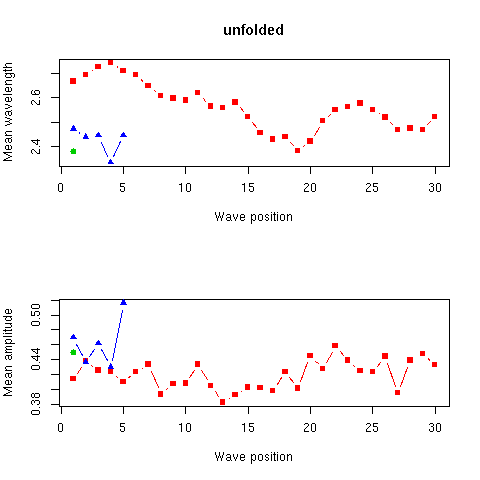
\includegraphics[width=1.0\textwidth]{figunfold.png}
%   wavlamplunfoldedisfc.png is original 
  \caption{Mean wavelength and amplitude at each wave position for all sheep with unfolded crimp type. The thirty red points represent the single fibre technique, the single green point the in-staple technique, and the five blue points the fibre-mount technique.}
  \label{fig:unfold}
\end{figure}

%\end{document}


%\documentclass{article}
%\usepackage{graphicx,subfigure}
%\begin{document}

\begin{figure}[!h]
  \centering
  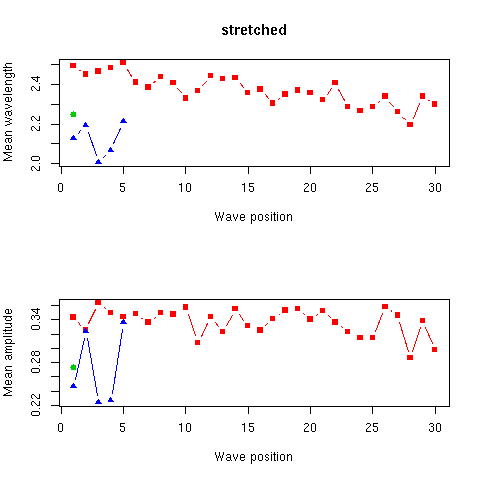
\includegraphics[width=1.0\textwidth]{figstretch.png}
%   wavlamplstretchedisfc.png is original 
  \caption{Mean wavelength and amplitude at each wave position for all sheep with stretched crimp type. The thirty red points represent the single fibre technique, the single green point the in-staple technique, and the five blue points the fibre-mount technique.}
  \label{fig:stretch}
\end{figure}

%\end{document}


%\documentclass{article}
%\usepackage{graphicx,subfigure}
%\begin{document}

\begin{figure}[!h]
  \centering
  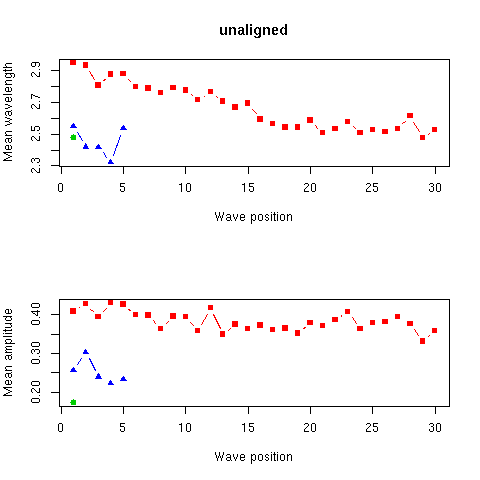
\includegraphics[width=1.0\textwidth]{figunalign.png}
%   wavlamplunalignedisfc.png is original 
  \caption{Mean wavelength and amplitude at each wave position for all sheep with unaligned crimp type. The thirty red points represent the single fibre technique, the single green point the in-staple technique, and the five blue points the fibre-mount technique.}
  \label{fig:unalign}
\end{figure}

%\end{document}



For wools of the {\em unfolded} crimp type, the IS and FC techniques appear to measure a smaller wavelength, and a slightly larger amplitude, compared to the SF technique.

For wools of the {\em stretched} and {\em unaligned} crimp types, the IS and FC techniques appear to measure a smaller wavelength and a smaller amplitude, compared to the SF technique.

The other issue is that all wools appear to decline in wavelength from base to tip ( as measured by the SF technique), but the {\em unaligned} wools appear to decline most in wavelength. Amplitude does not appear to change much from base to tip, for any of the three crimp types. This is in itself a puzzle. For wavelength to change without amplitude changing in a wave in a solid object like a fibre, the structure of the fibre must be changing. This could not happen with a simple stretch or relax.

These observations need to be confirmed by statistical testing. That is done in the following sections. We will defer further discussion until after that.

\clearpage
\section{Statistical comparison of techniques}
\subsection{Mean differences between techniques on base crimp wave}
A check on  differences between the three techniques was obtained by comparing the mean wavelength and amplitude of the base crimp wave for each sheep, the base crimp wave being the only wave position measured by all three techniques. Table ~\ref{tab:fwwavlaov} shows an anlaysis of variance of wavelength measured on the base crimp wave. 
%\documentclass{article}
%\usepackage{lscape}
%\begin{document}

\begin{table}[htp]
\centering
\caption{Analysis of variance of wavelength measured on the base crimp wave in a staple by three techniques (single-fibre, fibre-mount, and in-staple) for wools of three crimp types with several sheep representing each crimp type}
\label{tab:fwwavlaov}
\vspace{0.1in}
\begin{tabular}{|p{1.3in}|p{0.4in}|p{0.4in}|p{0.4in}|p{0.4in}|p{0.8in}|} \hline
     Source of Variation & Df & Sum Sq  & Mean Sq  & F Value  & Significance  \\  \hline
 Error: Sheep & & & & & \\
 CrimpType & 2 & 1.472 & 0.7361 & 0.254 & NS  \\
 Sheep/CrimpType & 18 & 8.946 & 0.4970 &  &  \\ 
 Error: Within & & & & & \\
 Technique & 2 & 1.364 & 0.6820 & 8.396  & ***  \\
 Residuals & 40 & 3.249 & 0.0812 & & \\ \hline
\end{tabular}
\end{table}

%\end{document}

This analysis of variance has two error levels, mean square for Sheep within CrimpType is the error for testing CrimpType, and mean square within subclasses is the error for testing Technique.
There were significant differences between Techniques. There was no interactions between Crimptype and Technique , so this term was omitted. What this means is that the Technique differences were consistent across all three CrimpTypes for wavelength. We need therefore only report the mean differences between Techniques , and this is done in Table~\ref{tab:fwmeans}.
%\documentclass{article}
%\usepackage{lscape}
%\begin{document}

\begin{table}[htp]
\centering
\caption{Effects of Technique and CrimpType on wavelength  measured on the base crimp wave in a staple by three techniques (single-fibre, fibre-mount, and in-staple) for wools of three crimp types with several sheep representing each crimp type}
\label{tab:fwmeans}
\vspace{0.1in}
\begin{tabular}{|p{1.8in}|p{1.0in}|p{0.9in}|} \hline
     Effect & Level & Wavelength (mm)  \\  \hline
 Mean       &       & 2.502         \\ \hline
 Technique & SF     & 2.709          \\
 Technique & FC     & 2.416     \\
 Technique & IS     & 2.381        \\ \hline
 CrimpType & unfolded &  2.502      \\
 CrimpType & stretched & 2.263      \\
 CrimpType & unaligned & 2.673      \\ \hline
\end{tabular}
\end{table}

%\end{document}

The single-fibre (SF) technique measures about 0.2 to 0.3 mm larger wavelength than the other two techniques.

An analysis of variance of amplitude measured on the base crimp wave is shown in Table~\ref{tab:fwamplaov}.
%\documentclass{article}
%\usepackage{lscape}
%\begin{document}

\begin{table}[htp]
\centering
\caption{Analysis of variance of amplitude measured on the base crimp wave in a staple by three techniques (single-fibre, fibre-mount, and in-staple) for wools of three crimp types with several sheep representing each crimp type}
\label{tab:fwamplaov}
\vspace{0.1in}
\begin{tabular}{|p{1.3in}|p{0.4in}|p{0.4in}|p{0.4in}|p{0.4in}|p{0.8in}|} \hline
     Source of Variation & Df & Sum Sq  & Mean Sq  & F Value  & Significance  \\  \hline
 Error: SheepNo & & & & & \\
 CrimpType & 2 & 0.04173 & 0.2086 & 15.66 & ***  \\
 Sheep/CrimpType & 18 & 0.2399 & 0.01333 &  &   \\ 
 Error: Within & & & & & \\
 Technique & 2 & 0.0418 & 0.02092 & 3.078  & $<$ 0.10  \\
 CrimpType:Technique & 4 & 0.1606 & 0.04016 & 5.908 & *** \\
 Residuals & 36 & 0.2447 & 0.00680 & & \\ \hline
\end{tabular}
\end{table}

%\end{document}

There is no significant overall difference between Techniques in amplitude ( significance level was 10 percent), but there is a significant difference between CrimpTypes. There was an interaction between Technique and CrimpType. What this means is that we should report the differences betwen Techniques separately for each CrimpType, and this is done in Table~\ref{tab:fameans}. 
%\documentclass{article}
%\usepackage{lscape}
%\begin{document}

\begin{table}[htp]
\centering
\caption{Effects of Technique and CrimpType on amplitude  measured on the base crimp wave in a staple by three techniques (single-fibre, fibre-mount, and in-staple) for wools of three crimp types with several sheep representing each crimp type}
\label{tab:fameans}
\vspace{0.1in}
\begin{tabular}{|p{1.0in}|p{1.0in}|p{0.9in}|} \hline
     Technique  & CrimpType & Amplitude (mm) \\  \hline
 Mean &  Mean       & 0.346  \\ \hline
 FC & stretched     & .246          \\
 FC & unaligned     & .255          \\
 FC & unfolded     &  .469          \\ \hline
 IS & stretched     & .273     \\
 IS & unaligned     & .173     \\
 IS & unfolded     &  .449     \\ \hline
 SF & stretched     & .324        \\
 SF & unaligned     & .388        \\
 SF & unfolded      & .401        \\ \hline
\end{tabular}
\end{table}

%\end{document}

We see that under the IS technique amplitude for the unaligned wools is smallest, whereas for the FC and SF techniques amplitude for the unaligned wools is intermediate. Also for the SF technique amplitude of the unaligned wools is very close to that for the unfolded wools, whereas for the FC technique it is close to that of the stretched wools. 

If we look at it the other way around, for unfolded wools the SF technique measures the smallest amplitude, wheareas for stretched and unaligned wools the SF technique measures the largest amplitude. 

We will leave the interpretation of this for later, but clearly the bias between techniques is not the same for all CrimpTypes. Not only is it not the same magnitude, it is in a different direction.




 -------- keep this for later
There are two possible reasons for this difference
\begin{itemize}
\item it may be related to the fibre being freed from its constraints within the staple. We know that the relaxed lengths of the fibres removed for the SF technique are longer on average than the staple length. For the relaxed length to increase, the crimp wavelengths would have to increase, but if that happened one would also expect the crimp amplitudes to decrease, and that did not happen.
\item it may be that the FC and IS techniques result in a biased sample of fibres being chosen for measurement, whereas the SF technique almost certainly measures a random sample of fibres. The FC and IS techniques would be likely to favour bundles of fibres that had their crimp waves in phase, and to ignore fibres not aligned with the dominant visible staple crimp.
\end{itemize}
 ---------

\subsection{Repeatability of base wave measurement across techniques}
\label{sec:repty}
It is one thing to compare techniques for bias, as in the previous Section. It is another to check if they rank samples in the same order. We do this by looking at the repeatability or correlation of measurements across the three techniques.

     For wavelength repeatability between the three techniques was highest between the IS and SF techniques (r=0.82), next best between the IS and FC techniques (r=0.69), and worst between the FC and SF techniques (r=0.52). Because the IS technique has replicate measures averaged ove five staples for the base crimp wave it is expected that it would have the best correlation. The IS x SF correlation is shown in Figure~\ref{fig:reptywavl}
%\documentclass{article}
%\usepackage{graphicx,subfigure}
%\begin{document}

\begin{figure}[!h]
  \centering
  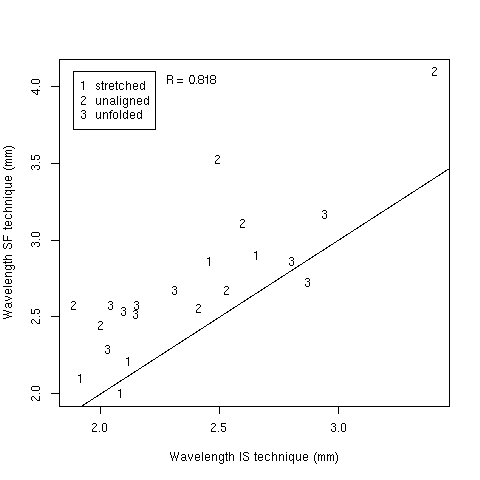
\includegraphics[width=1.0\textwidth]{figreptywavl.png}
%   reptywavl.png is original 
  \caption{Repeatebility between in-staple and single-fibre measurement techniques for wavelength}
  \label{fig:reptywavl}
\end{figure}

%\end{document}


The bias analysed in the previous Section is obvious, most points are above the 1 to 1 line, and there is a suggestion that the {\em unaligned} crimp type has a larger bias and poorer repeatability.

	For amplitude, repeatability between the three techniques was highest between the IS and FC techniques (r=0.74), next best between the IS and SF techniques (r=0.29), and worst between the FC and SF techniwues (r=0.18). However, because of the interaction between CrimpType and Technique for amplitude reported above, we really should do these correlations within CrimpTypes, so that the differential biases do not degrade the correlations. This is done in Table~\ref{tab:arepty}.
%\documentclass{article}
%\usepackage{lscape}
%\begin{document}

\begin{table}[htp]
\centering
\caption{Repeatability across techniques separately for each crimp type}
\label{tab:arepty}
\vspace{0.1in}
\begin{tabular}{|p{1.0in}|p{1.0in}|p{0.9in}|p{0.9in}} \hline
     CrimpType  & IS x SF & FC x SF & IS x FC \\  \hline
  stretched     & .092  & .861 & -.195   \\
  unaligned     & .714  & -.255 & .061  \\
  unfolded      & .412  & .227 &  .820\\ \hline
\end{tabular}
\end{table}

%\end{document}

We can see that these correlations are all over the place. There are clearly not enough replicate sheep within each crimp type to do these correlations separately.
	We finish with a plot of the IS x SF correlation for amplitude (Figure\ref{fig:reptyampl}. 

%\documentclass{article}
%\usepackage{graphicx,subfigure}
%\begin{document}

\begin{figure}[!h]
  \centering
  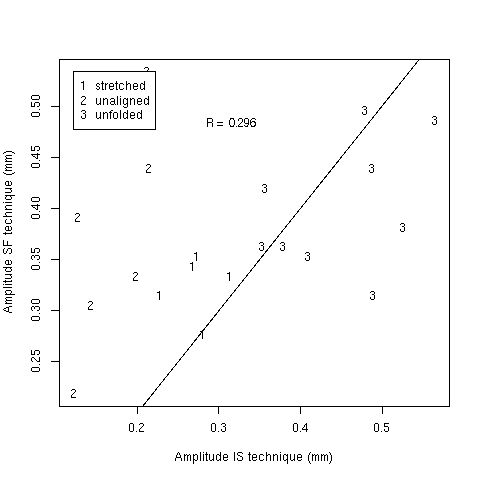
\includegraphics[width=1.0\textwidth]{figreptyampl.png}
%   reptyampl.png is original 
  \caption{Repeatebility between in-staple and single-fibre measurement techniques for amplitude}
  \label{fig:reptyampl}
\end{figure}

%\end{document}



The interaction analysed in the previous section is obvious, the {\em unaligned} wools measure higher with SF technique while the {\em unfolded} wools measure higher with IS technique. The overall repeatability is therefore a mixture of interacting biases and correlation, and is difficult to interpret.

In general it could be concluded that wavelength can be measured more repeatably than amplitude.  There is no technical difficulty in applying a ruler to a fibre image either for wavelength or crimp height. The issues with repeatability and bias have to be due to selection of which fibres to measure.

\subsection{The first five crimp waves from the staple base for SF and FC techniques only}
In the FC technique 5 successive waves from the staple base were measured, so it is possible to compare these 5 results with the first 5 waves from the base measured by the SF technique. This should result in a more accurate comparison than just using the one base wave. 

In analysing these data we have to consider  that the five successive waves will almost certainly have correlated measurement results.  The analysis of this is shown in Table~\ref{tab:wavl5} for wavelength.
%\documentclass{article}
%\usepackage{lscape}
%\begin{document}

\begin{table}[htp]
\centering
\caption{Analysis of variance of wavelength measured on the first five crimp waves in a staple by to techniques (single-fibre, fibre-mount) for wools of three crimp types with several sheep representing each crimp type}
\label{tab:wavl5}
\vspace{0.1in}
\begin{tabular}{|p{1.3in}|p{0.4in}|p{0.4in}|p{0.4in}|p{0.4in}|p{0.8in}|} \hline
     Source of Variation & Df & Sum Sq  & Mean Sq  & F Value  & Significance  \\  \hline
 Error: Sheep & & & & & \\
 CrimpType & 2 & 4.64 & 2.318 & 1.201 & NS  \\
 Sheep/CrimpType & 18 & 34.74 & 1.930 &  &  \\ 
 Error: Within & & & & & \\
 Technique & 1 & 6.169 & 6.169 & 134.8  & ***  \\
 WavNo & 4 & 0.202 & 0.050 & 1.102 & NS \\
 Residuals & 184 & 8.415 & 0.046 & & \\ \hline
\end{tabular}
\end{table}

%\end{document}

The only significant effect is Technique. There were no interactions Technique:CrimpType, Technique:WaveNo, or CrimpTYpe:WaveNo, so these were omitted. The Technique effect was a mean of 2.362 for FC and 2.704 for SF, a difference of about 0.34, similar to the base wave result.

The analysis for amplitude is shown in Table~\ref{tab:ampl5}
%\documentclass{article}
%\usepackage{lscape}
%\begin{document}

\begin{table}[htp]
\centering
\caption{Analysis of variance of amplitude measured on the first five crimp waves in a staple by to techniques (single-fibre, fibre-mount) for wools of three crimp types with several sheep representing each crimp type}
\label{tab:ampl5}
\vspace{0.1in}
\begin{tabular}{|p{1.3in}|p{0.4in}|p{0.4in}|p{0.4in}|p{0.4in}|p{0.8in}|} \hline
     Source of Variation & Df & Sum Sq  & Mean Sq  & F Value  & Significance  \\  \hline
 Error: Sheep & & & & & \\
 CrimpType & 2 & 0.7435 & 0.3717 & 7.37 & NS  \\
 Sheep/CrimpType & 18 & 0.9078 & 0.504 &  &  \\ 
 Error: Within & & & & & \\
 Technique & 1 & 0.0891 & 0.089 & 10.63  & **  \\
 WavNo & 4 & 0.0299 & 0.00748 & 0.893 & NS \\
 Technique:CrimpType & 2 & 0.4242 & 0.2123 & 25.35 & *** \\
 Residuals & 182 & 1.5241 & 0.00837 & & \\ \hline
\end{tabular}
\end{table}

%\end{document}

For amplitude the significant effects are Technique and the interaction Technique:CrimpType,  as for the single base wave analysis. This means that we must look at the Technique difference separately for each CrimpType, and this is done in Table~\ref{tab:ampl5means}
%\documentclass{article}
%\usepackage{lscape}
%\begin{document}

\begin{table}[htp]
\centering
\caption{Effects of Technique and CrimpType on amplitude  measured on the first fice crimp waves in a staple by two techniques (single-fibre, fibre-mount) for wools of three crimp types with several sheep representing each crimp type}
\label{tab:ampl5means}
\vspace{0.1in}
\begin{tabular}{|p{1.0in}|p{1.0in}|p{0.9in}|} \hline
     Technique  & CrimpType & Amplitude (mm) \\  \hline
 Mean &  Mean       & 0.366  \\ \hline
 FC & stretched     & .27          \\
 FC & unaligned     & .25          \\
 FC & unfolded     &  .46          \\ \hline
 SF & stretched     & .33        \\
 SF & unaligned     & .30        \\
 SF & unfolded      & .41        \\ \hline
\end{tabular}
\end{table}

%\end{document}

We can see that the SF technique again measures a larger amplitude for the stretched and unaligned wools, and a smaller amplitude for the unfolded wools.

\subsection{The first 20 base waves and the last 10 tip waves for single-fibre technique only}
\label{sf2010}
There is actually much more data available for the SF technique than we have looked at so far. There are measurements of wavelength and amplitude on the first 20 successive waves from the staple base, and on the last 10 succesive waves ending at the staple tip. There is no Technique comparison here, but it is obvious from Figures~\ref{fig:unfold}, \ref{fig:stretch}, and ~\ref{fig:unalign}, that the profile of wavelengths and amplitudes along the staple is different for the three CrimpTypes. There is also the question of why wavelength and amplitude should vary along the staple, and the implicatins of this for sampling and measurement of crimp. We should also look at single fibre data rather than the means graphes in Figures~\ref{fig:unfold}, \ref{fig:stretch}, and ~\ref{fig:unalign}, because each fibre is the statistical 'Block' within which a sequence of successive waves are measured.

\subsubsection{The raw data}
Before doing an analysis, we will just look at some of the raw data on individual fibres. Figure~\ref{fig:sfwavl} shows the wavelength measurements for each of 15 fibres from sheep number 9. 
%\documentclass{article}
%\usepackage{graphicx,subfigure}
%\begin{document}

\begin{figure}[!h]
  \centering
  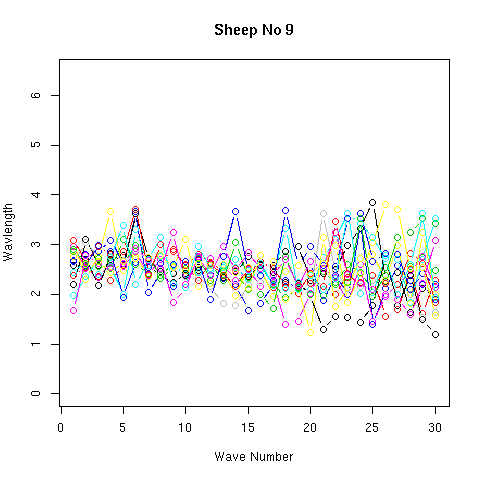
\includegraphics[width=1.0\textwidth]{figsfwavl.png}
%   sheep9wavl.png is original 
  \caption{Wavelength measured along 15 fibres for sheep no 9.}
  \label{fig:sfwavl}
\end{figure}

%\end{document}


It can be seem that the wavelengths are quite variable both along the fibre and between fibres, the between fibre variabiltiy seems to increase towards the tip of the staple, and the mean wavelength declines towards the staple tip. This is a 'typical' sheep, there are some more variable, some less.

Figure~\ref{fig:sfampl} shows the amplitude measurements for each of 15 fibres from sheep number 9.
%\documentclass{article}
%\usepackage{graphicx,subfigure}
%\begin{document}

\begin{figure}[!h]
  \centering
  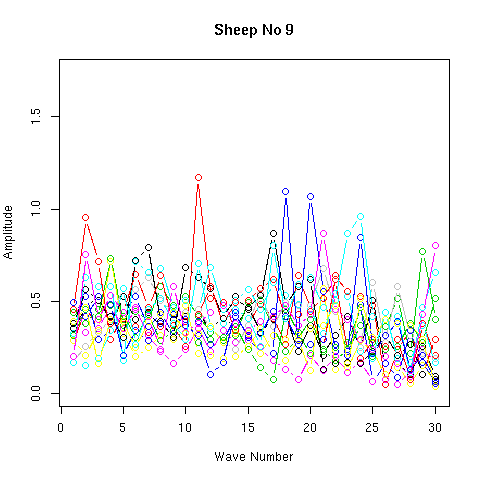
\includegraphics[width=1.0\textwidth]{figsfampl.png}
%   sheep9ampl.png is original 
  \caption{Amplitude measured along 15 fibres for sheep no 9.}
  \label{fig:sfampl}
\end{figure}

%\end{document}


The amplitude data are more variable than the wavelength data, both between and along fibres. For this sheep, the amplitude declines toward the staple tip. Other sheep are also quite variable and it is difficlut to say what is typical.

We proceed to an analysis of variance of the full SF technique data with 21 sheep, 15 fibres per sheep and 30 waves per fibre measured for both wavelength and amplitude.

\subsubsection{Variance components}
We will first do an analysis considering  the 30 waves per fibre  to be a random sample of waves despite their sequential nature, and the SheepNo and FibreNo effects also being considered random. The resulting  analysis of variance for wavelength is shown in Table~\ref{tab:sfwavlaov}.
%\documentclass{article}
%\usepackage{lscape}
%\begin{document}

\begin{table}[htp]
\centering
\caption{Analysis of variance of wavelength (mm) measured on 15 sheep with 15 fibres per sheep and 30 waves per fibre. Wools were of three crimp types with several sheep representing each crimp type}
\label{tab:sfwavlaov}
\vspace{0.1in}
\begin{tabular}{|p{1.4in}|p{0.4in}|p{0.4in}|p{0.4in}|p{0.4in}|p{0.8in}|} \hline
     Source of Variation & Df & Sum Sq  & Mean Sq  & F Value  & Significance  \\  \hline
 CrimpType & 2 & 115.4 & 57.72 & 0.95 & NS  \\
 SheepNo/CrimpType & 18 & 1085.3 & 49.01 &  49.01 & ***    \\ 
 FibreNo/SheepNo & 294 & 361.7 & 1.23 & 5.48 & ***  \\
 Residuals (WaveNo/FibreNo) & 9135 & 2047.8 & 0.224 & & \\ \hline
\end{tabular}
\end{table}

%\end{document}

The Residual effect in Table~\ref{tab:sfwavlaov} is WaveNo within FibreNo.
There were significant effects for  Sheep within CrimpType  and Fibres within Sheep, but we are mainly interested in the variances.  

The mean squares for each effect in Table~\ref{tab:sfwavlaov} can be equated to their expectations in terms of variance components as shown in Table~\ref{tab:ems}.
%\documentclass{article}
%\usepackage{lscape}
%\begin{document}

\begin{table}[htp]
\centering
\caption{Expected values of mean squares for the analysis of Table~\ref{tab:sfwavlaov} in terms of variance components for SheepNo/CrimpType ($\sigma^{2}_{S}$), FibreNo/SheepNo  ($\sigma^{2}_{F}$), and WaveNo/FibreNo ($\sigma^{2}_{W}$).}
\label{tab:ems}
\vspace{0.1in}
\begin{tabular}{|p{1.4in}|p{2.4in}|} \hline
     Mean square & Expectation    \\  \hline
 SheepNo/CrimpType & $\sigma^{2}_{W} + 30 \sigma^{2}_{F} + 450 \sigma^{2}_{S}$     \\ 
 FibreNo/SheepNo & $\sigma^{2}_{W} + 30 \sigma^{2}_{F}$   \\
 WaveNo/FibreNo & $\sigma^{2}_{W}$  \\ \hline
\end{tabular}
\end{table}

%\end{document}

We have in Table~\ref{tab:ems} 3 equations in 3 unknowns so we can solve them to obtain estimates of the variance components as follows
\begin{eqnarray*}
\sigma^{2}_{W} & = & MS(WaveNo/FibreNo) \\
\sigma^{2}_{F} & = & [MS(FibreNo/SheepNo) - MS(WaveNo/FibreNo)]/30 \\
\sigma^{2}_{S} & = & [MS(SheepNo/CrimpType) - MS(FibreNo/SheepNo)]/450 
\end{eqnarray*}

For wavelength these calculations result in the following estimates for variance components
\begin{eqnarray*}
\sigma^{2}_{W} & = & 0.224 \\
\sigma^{2}_{F} & = & 0.0337 \\
\sigma^{2}_{S} & = & 0.131
\end{eqnarray*}
all in units of $mm^{2}$.
We can use these variance component estimates to assess the errors of measurement of wavelength obtained by measuring various numbers of fibres per sheep and waves per fibre. For example measuring 10 fibres per sheep and 20 waves per fibre we obtain a sample variance of wavelength of $\sigma^{2}_{F}/10 + \sigma^{2}_{W}/20$ which is $.0337/10 + .224/20 = 0.0145$.
This corresponds to a standard error of measurement of wavelength of $\sqrt(0.0145 ) = 0.12$.
The larger variance component ($\sigma^{2}_{W}$) contributes most to the measurement error.

We now do the same all random analysis for amplitude. The resulting  analysis of variance for wavelength is shown in Table~\ref{tab:sfamplaov}.
%\documentclass{article}
%\usepackage{lscape}
%\begin{document}

\begin{table}[htp]
\centering
\caption{Analysis of variance of amplitude (mm) measured on 15 sheep with 15 fibres per sheep and 30 waves per fibre. Wools were of three crimp types with several sheep representing each crimp type}
\label{tab:sfamplaov}
\vspace{0.1in}
\begin{tabular}{|p{1.4in}|p{0.4in}|p{0.4in}|p{0.4in}|p{0.4in}|p{0.8in}|} \hline
     Source of Variation & Df & Sum Sq  & Mean Sq  & F Value  & Significance  \\  \hline
 CrimpType & 2 & 10.02 & 5.011 & 1.43 & NS  \\
 SheepNo/CrimpType & 18 & 62.77 & 3.487 &  14.83 & ***    \\ 
 FibreNo/SheepNo & 294 & 69.15 & 0.235 & 8.02 & ***  \\
 Residuals (WaveNo/FibreNo) & 9135 & 268.27 & 0.0293 & & \\ \hline
\end{tabular}
\end{table}

%\end{document}

The Residual effect in Table~\ref{tab:sfamplaov} is WaveNo within FibreNo.
There were significant effects for  Sheep within CrimpType  and Fibres within Sheep, as for wavelength. 
The expected mean squares of Table~\ref{tab:ems} apply also to amplitude, so we can again solve the 3 equiations to obtain variance component estimates as follows
\begin{eqnarray*}
\sigma^{2}_{W} & = & 0.0293 \\
\sigma^{2}_{F} & = & 0.00685 \\
\sigma^{2}_{S} & = & 0.00722
\end{eqnarray*}
all in units of $mm^{2}$.

Again, $\sigma^{2}_{W}$ is larger than $\sigma^{2}_{F}$ and contributes most to error of measurement.

\subsubsection{Variance components adjusted for systematic differences between Regions of the staple}
We know from Figures~\ref{fig:unfold}, \ref{fig:stretch}, and ~\ref{fig:unalign} that there are trends along the staple in wavelength, and to a lesser extent in amplitude in these data. There exists the possibility that we could reduce the WaveNo/FibreNo variance component ($\sigma^{2}_{W}$) by choosing to measure within a nominated part of the staple length, rather than all along it as in our series of 30 measurements.
 To this end we need to re-estimate what $\sigma^{2}_{W}$ would be if we take out the variation between staple regions. To do this we define a Region effect and add it to the analysis of variance. We define Region to be
\begin{description}
\item[base] first 10 waves from staple base
\item[mid] next 10 waves
\item[tip] last 10 waves from staple tip
\end{description}

An analysis of variance of wavelength, including a Region effect and its interactions, is given in Table~\ref{tab:sfwavlaovreg}.
%\documentclass{article}
%\usepackage{lscape}
%\begin{document}

\begin{table}[htp]
\centering
\caption{Analysis of variance of wavelength (mm) measured on 15 sheep with 15 fibres per sheep and 30 waves per fibre. Wools were of three crimp types with several sheep representing each crimp type. An effect of Region has been introduced to remove any systematic variation along the staple from the variance of WaveNo within FibreNo.}
\label{tab:sfwavlaovreg}
\vspace{0.1in}
\begin{tabular}{|p{1.4in}|p{0.4in}|p{0.4in}|p{0.4in}|p{0.4in}|p{0.8in}|} \hline
     Source of Variation & Df & Sum Sq  & Mean Sq  & F Value  & Significance  \\  \hline
 CrimpType & 2 & 115.4 & 57.72 & 0.95 & NS  \\
 SheepNo/CrimpType & 18 & 1085.3 & 49.01 &  49.01 & ***    \\ 
 FibreNo/SheepNo & 294 & 361.7 & 1.23 & 5.48 & ***  \\
 Region & 2 & 67.0 & 33.49 & 155.3 &  *** \\
 CrimpType:Region & 4 & 12.6 & 3.16 & 14.6 & *** \\
 Residuals (WaveNo/FibreNo) & 9129 & 1968.8 & 0.216 & & \\ \hline
\end{tabular}
\end{table}

%\end{document}

It can be seen that the Region effect takes an amount of 67.0 out of the sum of squares for Residual, and the CrimpType:Region interaction takes a further 12.6. This reduces the Residual sum of squares for 2047.8 in Table~\ref{tab:sfwavlaov} to 1968.2 in Table~\ref{tab:sfwavlaovreg}. The mean square for Residual is reduced from 0.114 to 0.216, a very small change. The effect on standard error of wavelength measurement of confining measurement to one Region would therefore be quite small.

The CrimpType:Region interaction is shown in Table~\ref{tab:sfwavlint}, along with the means for each CrimpTYpe and each Region.
%\documentclass{article}
%\usepackage{lscape}
%\begin{document}

\begin{table}[htp]
\centering
\caption{Effects of CrimpType and Region on wavelength  measured on 30 waves per fibre by the single-fibre technique for wools of three crimp types with several sheep representing each crimp type}
\label{tab:sfwavlint}
\vspace{0.1in}
\begin{tabular}{|p{1.0in}|p{1.0in}|p{0.9in}|} \hline
     CrimpType  & Region & Wavelength (mm) \\  \hline
 Mean &  Mean       & 2.551  \\ \hline
  stretched     & base & 2.435          \\
  unaligned     & base & 2.833          \\
  unfolded     &  base & 2.667          \\ \hline
  stretched     & mid & 2.377     \\
  unaligned     & mid & 2.636     \\
  unfolded     &  mid & 2.497     \\ \hline
  stretched     & tip & 2.299        \\
  unaligned     & tip & 2.530        \\
  unfolded      & tip & 2.520        \\ \hline
  stretched     & mean & 2.371 \\
  unaligned     & mean & 2.666 \\
  unfolded      & mean & 2.561 \\ \hline
  mean          & base & 2.667 \\
  mean          & mid  & 2.515 \\
  mean          & tip  & 2.471 \\ \hline
\end{tabular}
\end{table}

%\end{document}

The interaction is small. For all CrimpTypes the wavelength declines from base to tip, so there is no reversal of rank, just a varying rate of decline with the unaligned wools declining most. Most of the decline is between the base and mid regions. 

An analysis of variance of amplitude, including a Region effect and its interactions, is given in Table~\ref{tab:sfamplaovreg}.
%\documentclass{article}
%\usepackage{lscape}
%\begin{document}

\begin{table}[htp]
\centering
\caption{Analysis of variance of amplitude (mm) measured on 15 sheep with 15 fibres per sheep and 30 waves per fibre. Wools were of three crimp types with several sheep representing each crimp type. An effect of Region has been introduced to remove any systematic variation along the staple from the variance of WaveNo within FibreNo.}
\label{tab:sfamplaovreg}
\vspace{0.1in}
\begin{tabular}{|p{1.4in}|p{0.4in}|p{0.4in}|p{0.4in}|p{0.4in}|p{0.8in}|} \hline
     Source of Variation & Df & Sum Sq  & Mean Sq  & F Value  & Significance  \\  \hline
 CrimpType & 2 & 10.02 & 5.011 & 1.43 & NS  \\
 SheepNo/CrimpType & 18 & 62.77 & 3.487 &  14.83 & ***    \\ 
 FibreNo/SheepNo & 294 & 69.15 & 0.235 & 8.02 & ***  \\
 Region & 2 & 0.49 & 0.243 & 8.32 &  *** \\
 CrimpType:Region & 4 & 0.82 & 0.204 & 6.97 & *** \\
 Residuals (WaveNo/FibreNo) & 9129 & 266.96 & 0.0292 & & \\ \hline
\end{tabular}
\end{table}

%\end{document}

There is a Region effect, and an interaction of CrimpType:Region, but they are small and remove little from the Residual mean square. There would be practically no effect on standard error of amplitude measurement of confining measurement to one Region.
The CrimpType:Region interaction is shown in Table~\ref{tab:sfamplint}, along with the means for each CrimpType and each Region.
%\documentclass{article}
%\usepackage{lscape}
%\begin{document}

\begin{table}[htp]
\centering
\caption{Effects of CrimpType and Region on amplitude  measured on 30 waves per fibre by the single-fibre technique for wools of three crimp types with several sheep representing each crimp type}
\label{tab:sfamplint}
\vspace{0.1in}
\begin{tabular}{|p{1.0in}|p{1.0in}|p{0.9in}|} \hline
     CrimpType  & Region & Amplitude (mm) \\  \hline
 Mean &  Mean       & 0.387  \\ \hline
  stretched     & base & 0.347          \\
  unaligned     & base & 0.404          \\
  unfolded     &  base & 0.417          \\ \hline
  stretched     & mid & 0.338     \\
  unaligned     & mid & 0.369     \\
  unfolded     &  mid & 0.409     \\ \hline
  stretched     & tip & 0.327        \\
  unaligned     & tip & 0.374        \\
  unfolded      & tip & 0.433        \\ \hline
  stretched     & mean & 0.337 \\
  unaligned     & mean & 0.382 \\
  unfolded      & mean & 0.420 \\ \hline
  mean          & base & 0.396 \\
  mean          & mid &  0.378 \\
  mean          & tip &  0.388 \\ \hline
\end{tabular}
\end{table}

%\end{document}

The amplitude declines from base to mid region, then increases slightly to the tip region.

\subsubsection{Are the successive wave measurements autocorrelated?}
The above variance component analyses assume that measurements on successive waves are not more highly correlated than measurements on pairs of waves chosen at random from anywhere along the staple. This needs to be investigated.

What we can do is compute the average correlation between successive waves for each fibre. This is referred to in time series analysis as an autocorrelation of lag=1. We can also do it for longer lags. In what follows we look at lags up to 10.

We first look at the autocorrelations for wavelength measurements for two individual fibres. These are shown as plots of correlation against lag in Figure~\ref{fig:acf}.
%\documentclass{article}
%\usepackage{graphicx,subfigure}
%\begin{document}

\begin{figure}[!h]
  \centering
  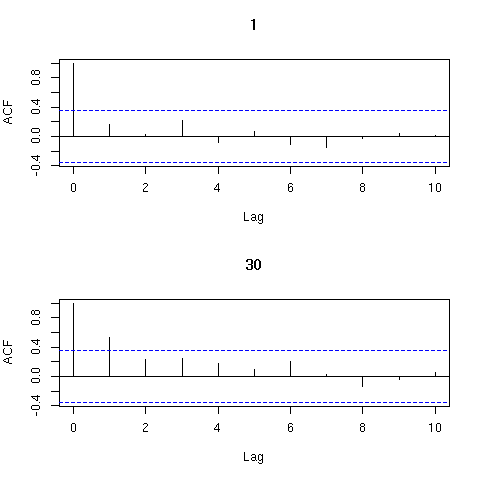
\includegraphics[width=1.0\textwidth]{figacf.png}
%   acffib.1.30.png is original 
  \caption{Autocorrelations for lags up to 10 for wavelength measurements on two individual fibres}
  \label{fig:acf}
\end{figure}

%\end{document}


The two fibres shown are fibre 1 ( the first fibre from the first sheep) and fibre 30 ( the last fibre from the second sheep). The autocorrelation for lag zero is, of course, always 1. For fibre 1, there are no significant autocorrelations - all the graph points fall inside the blue lines. This is typical - most fibres are like this. For fibre 30 the lag 1 autocorrelation is significant and positive, and all the autocorrelations tend to decline with increasing lag. This is not typical - only a few fibres are like this.

We cant show the whole 315 fibres as plots. What we have done is to compute the lag 1 to lag 10 autocorrelations for each fibre, then pool them ( using Fisher's z transformation) to give the average autocorrelation for each sheep, and overall. We did this for both wavelength and amplitude. The results are shown in Tables~\ref{tab:acfw} and \ref{tab:acfa}.
% latex table generated in R 3.2.4 by xtable 1.8-2 package
% Tue Jul 26 19:41:01 2016
\begin{table}[htp]
\centering
\caption{Autocorrelations for wavelength along individual fibres, for lags 1 to 10,  pooled across 15 fibres for each sheep, and overall}
\label{tab:acfw}
\vspace{0.1in}
\begin{tabular}{rrrrrrrrrrrr}
  \hline
 Lags & 1 & 2 & 3 & 4 & 5 & 6 & 7 & 8 & 9 & 10  \\ 
  \hline
Sheep 1 &   0.02 & 0.05 & -0.01 & 0.02 & -0.06 & -0.02 & -0.01 & -0.08 & 0.02 & -0.00 \\ 
Sheep 2   & 0.26 & 0.20 & 0.17 & 0.15 & 0.12 & 0.01 & 0.03 & -0.03 & -0.03 & -0.01 \\ 
Sheep 3   & 0.27 & 0.10 & 0.04 & -0.01 & -0.03 & -0.02 & -0.05 & -0.03 & -0.10 & -0.07 \\ 
Sheep 4   & 0.13 & 0.09 & 0.01 & 0.02 & -0.05 & -0.03 & -0.01 & -0.09 & -0.11 & -0.07 \\ 
Sheep 5   & 0.02 & -0.09 & 0.05 & -0.05 & -0.07 & -0.02 & -0.03 & 0.01 & -0.03 & -0.04 \\ 
Sheep  6   & 0.29 & 0.20 & 0.06 & 0.08 & 0.04 & 0.08 & -0.01 & 0.04 & -0.01 & -0.01 \\ 
Sheep  7   & 0.12 & 0.06 & 0.09 & 0.00 & -0.00 & 0.01 & -0.06 & -0.07 & -0.10 & -0.06 \\ 
Sheep  8   & 0.16 & 0.02 & -0.06 & -0.08 & -0.01 & -0.07 & -0.05 & -0.02 & -0.03 & 0.01 \\ 
Sheep  9   & 0.21 & 0.15 & 0.06 & 0.05 & 0.06 & 0.02 & -0.02 & -0.04 & 0.01 & -0.05 \\ \hline
Sheep  10   & 0.09 & -0.02 & -0.02 & -0.03 & -0.11 & -0.07 & -0.07 & -0.01 & -0.08 & -0.06 \\ 
Sheep  11   & 0.24 & 0.16 & 0.13 & 0.00 & 0.01 & -0.03 & -0.01 & 0.00 & 0.03 & -0.02 \\ 
Sheep  12   & 0.20 & 0.12 & 0.12 & 0.02 & -0.03 & -0.06 & 0.05 & -0.05 & -0.01 & 0.02 \\ 
Sheep  13   & 0.17 & 0.09 & 0.06 & 0.07 & 0.01 & -0.03 & 0.00 & -0.04 & -0.03 & -0.02 \\ 
Sheep  14   & 0.15 & 0.04 & -0.07 & -0.03 & -0.01 & -0.08 & 0.03 & -0.04 & -0.02 & -0.02 \\ 
Sheep  15   & 0.20 & 0.06 & 0.06 & -0.02 & -0.01 & -0.02 & 0.00 & 0.04 & 0.13 & -0.08 \\  \hline
Sheep  16   & 0.20 & 0.02 & 0.13 & 0.12 & 0.00 & 0.06 & -0.06 & -0.02 & -0.00 & -0.05 \\ 
Sheep  17   & 0.07 & 0.06 & 0.05 & -0.02 & -0.04 & -0.05 & -0.02 & -0.03 & -0.00 & -0.09 \\ 
Sheep  18   & 0.17 & 0.08 & 0.11 & 0.03 & 0.09 & 0.09 & -0.02 & -0.05 & 0.03 & -0.05 \\ 
Sheep  19   & 0.02 & -0.01 & 0.01 & -0.06 & -0.05 & -0.06 & -0.00 & -0.02 & -0.03 & -0.03 \\ 
Sheep  20   & 0.37 & 0.26 & 0.21 & 0.10 & 0.17 & 0.10 & -0.00 & 0.01 & -0.06 & -0.04 \\ 
Sheep  21   & 0.18 & 0.00 & 0.07 & 0.03 & -0.02 & -0.02 & 0.04 & -0.01 & -0.03 & -0.13 \\ 
   \hline
Overall &  0.17 & 0.08 & 0.06 & 0.02 & 0.00 & -0.01 & -0.01 & -0.03 & -0.02 & -0.04 \\ \hline
\end{tabular}
\end{table}

% latex table generated in R 3.2.4 by xtable 1.8-2 package
% Tue Jul 26 19:41:30 2016
\begin{table}[htp]
\centering
\caption{Autocorrelations for amplitude along individual fibres, for lags 1 to 10,  pooled across 15 fibres for each sheep, and overall}
\label{tab:acfa}
\vspace{0.1in}
\begin{tabular}{rrrrrrrrrrrr}
  \hline
 & 1 & 2 & 3 & 4 & 5 & 6 & 7 & 8 & 9 & 10  \\ 
  \hline
Sheep 1   & 0.00 & 0.06 & 0.09 & 0.00 & 0.05 & -0.05 & 0.04 & -0.02 & -0.06 & 0.01 \\ 
Sheep  2   & 0.05 & 0.08 & 0.03 & 0.15 & 0.04 & 0.00 & -0.03 & -0.00 & 0.01 & -0.03 \\ 
Sheep  3   & 0.17 & 0.10 & -0.00 & 0.05 & -0.03 & -0.01 & -0.06 & 0.03 & -0.02 & -0.05 \\ 
Sheep  4   & 0.01 & 0.00 & 0.04 & 0.01 & -0.06 & -0.06 & 0.05 & -0.01 & 0.02 & -0.00 \\ 
Sheep  5   & -0.02 & 0.00 & 0.04 & 0.04 & -0.03 & 0.10 & -0.07 & -0.04 & 0.02 & -0.05 \\ 
Sheep  6   & 0.15 & 0.07 & 0.03 & 0.06 & -0.00 & -0.01 & 0.03 & 0.04 & -0.04 & 0.00 \\ 
Sheep  7   & 0.17 & 0.14 & 0.07 & 0.05 & 0.02 & 0.04 & -0.00 & -0.03 & 0.00 & -0.04 \\ 
Sheep  8   & -0.13 & 0.12 & -0.08 & 0.02 & 0.02 & 0.04 & -0.06 & 0.07 & -0.10 & -0.02 \\ 
Sheep  9   & 0.21 & 0.15 & 0.11 & 0.10 & 0.02 & 0.04 & -0.04 & -0.05 & 0.00 & -0.04 \\  \hline
Sheep  10   & -0.01 & -0.01 & -0.03 & 0.00 & -0.08 & -0.04 & 0.01 & -0.06 & -0.07 & -0.01 \\ 
Sheep  11   & 0.17 & 0.10 & 0.06 & -0.00 & 0.02 & 0.02 & 0.00 & -0.03 & -0.05 & -0.05 \\ 
Sheep  12   & -0.02 & 0.05 & 0.09 & 0.05 & 0.02 & -0.04 & 0.08 & -0.05 & -0.03 & 0.00 \\ 
Sheep  13   & 0.01 & 0.07 & -0.02 & -0.05 & 0.03 & 0.01 & 0.02 & 0.01 & -0.05 & -0.00 \\ 
Sheep  14   & 0.15 & 0.11 & 0.08 & 0.01 & 0.02 & -0.07 & 0.03 & -0.02 & -0.05 & -0.09 \\ 
Sheep  15   & -0.00 & -0.03 & -0.02 & -0.07 & 0.04 & -0.03 & -0.06 & -0.06 & 0.07 & -0.07 \\  \hline
Sheep  16   & 0.06 & 0.01 & 0.07 & 0.10 & 0.02 & 0.10 & -0.01 & 0.03 & -0.03 & -0.04 \\ 
Sheep  17   & -0.08 & 0.01 & 0.04 & -0.05 & 0.00 & 0.03 & -0.00 & -0.04 & 0.05 & -0.07 \\ 
Sheep  18   & 0.03 & -0.04 & 0.06 & 0.01 & 0.08 & 0.03 & -0.08 & -0.06 & 0.07 & 0.01 \\ 
Sheep  19   & 0.11 & 0.06 & 0.14 & 0.14 & 0.03 & -0.00 & 0.02 & -0.02 & -0.05 & -0.06 \\ 
Sheep  20   & 0.16 & 0.06 & 0.08 & -0.04 & 0.01 & -0.09 & -0.08 & 0.00 & -0.18 & -0.08 \\ 
Sheep  21   & 0.04 & 0.01 & 0.11 & 0.01 & -0.06 & -0.03 & 0.03 & -0.05 & -0.10 & -0.01 \\ 
   \hline
Overall & 0.06 & 0.05 & 0.04 & 0.03 & 0.01 & -0.00 & -0.01 & -0.02 & -0.03 & -0.03 \\ \hline
\end{tabular}
\end{table}

For wavelength, the autocorrelations are small for all sheep. Sheep 20 has the largest, but 0.37 is still not significant. The overall pooled result shows a good summary - the correlations are tiny and decline graduallly with increasing lag.
For amplitude the result is similar but with autocorrelations being generally smaller than for wavelength.

The conclusion is therefore quite clear. There is no need to worry about the observations fron the SF technique being serially correlated. There is no evidence of any significant autocorrelation. The variance component analyses above, which assume each wave to be an independent random sample from a population of waves, are therefore correct.

Perhaps this result is surprising. We all know that successive crimp waves are similar in wavelength and amplitude, but that is not the point. The point is that the errors of measuring them are not serially correlated.


\subsubsection{The relationship between wavelength and amplitude}
There is an opportunity to use the extensive data from the SF technique to look at whether wavelength and amplitude are correlated either within a fibre, or between fibres, or between sheep. 

Before proceeding we need to remember that stretched helix crimp and unfolded helix crimp are formed in different ways and that the relationship (if any) observed between wavelength and amplitude measured in the staple may not be the same for these two crimptypes. 

Remember that the biological parameters are intrinsic curvature and fibre length growth rate. For a stretched helix wool length growth rate determines the amount of 'stretch' which is the wavelength, while intrinsic curvature and wavelength both determine the observed amplitude which will be similar to intrinsic curvature but slightly smaller, depending on the amount of 'stretch'.

For unfolded helix wools, amplitude is greater than intrinsic radius when the angle between unfoldings exceeds 180 degrees ( ie in horseshoe crimp wools), is less than intrinsic radius when the angle between unfoldings is less then 180 degrees, and is equal to intrinsic radius when the angle between unfoldings is equal to 180 degrees.  Wavelength depends on intrinsic radius and angle between unfoldings, not on length growth rate.

So the situation is complicated, and we should look carefully for any effect of crimptype.

There can be correlations between wavelength and amplitude at various levels
\begin{itemize}
\item between sheep within crimptypes
\item between fibres within sheep
\item between waves within fibres
\end{itemize}
To calculate each of these correlations we need to do an analysis of covariance and calculate covariance components ( ie covariances between wavelength and amplitude for each of the above levels). We do this by the time-honoured method of doing an analysis of variance of the sum of wavelength and amplitude. This works because of the following identity
\begin{displaymath}
Var(A + B) = Var(A) + Var(B) + 2 Cov(A,B)
\end{displaymath}
which can be turned around to calculate a covariance as
\begin{displaymath}
Cov(A,B) = [Var(A + B) - Var(A) -  Var(B)]/2
\end{displaymath}

So in our case we start with an analysis of variance of the sum of wavelength and amplitude along the same lines as the analyses for wavelength and amplitude in Figures~\ref{tab:sfwavlaov} and \ref{tab:sfamplaov}. Then we apply the above identity to the mean squares and obtain an analysis of covariance table given in Table~\ref{tab:sfwavlamplancov}.

%\documentclass{article}
%\usepackage{lscape}
%\begin{document}

\begin{table}[htp]
\centering
\caption{Analysis of covariance of wavelength and amplitude measured on 15 sheep with 15 fibres per sheep and 30 waves per fibre. Wools were of three crimp types with several sheep representing each crimp type}
\label{tab:sfwavlamplancov}
\vspace{0.1in}
\begin{tabular}{|p{1.4in}|p{0.4in}|p{0.7in}|p{0.4in}|p{0.8in}|} \hline
     Source of Variation & Df &  Mean Product  & F Value  & Significance  \\  \hline
 CrimpType & 2 &  9.972 & 0.72 & NS  \\
 SheepNo/CrimpType & 18 &   13.8215 &  40.19 & ***    \\ 
 FibreNo/SheepNo & 294 &  0.3425 & 8.99 & ***  \\
 Residuals (WaveNo/FibreNo) & 9135 &  0.03823 & & \\ \hline
\end{tabular}
\end{table}

%\end{document}


The mean products for each effect in Table~\ref{tab:sfwavlamplancov} can be equated to their expectations in terms of covariance components as shown ( for variance components) in Table~\ref{tab:ems}.

We have in Table~\ref{tab:ems} 3 equations in 3 unknowns so we can solve them to obtain estimates of the covariance components as follows
\begin{eqnarray*}
\sigma_{W} & = & MP(WaveNo/FibreNo) \\
\sigma_{F} & = & [MP(FibreNo/SheepNo) - MP(WaveNo/FibreNo)]/30 \\
\sigma_{S} & = & [MP(SheepNo/CrimpType) - MP(FibreNo/SheepNo)]/450
\end{eqnarray*}

For wavelength and amplitude these calculations result in the following estimates for covariance components
\begin{eqnarray*}
\sigma_{W} & = & 0.03823 \\
\sigma_{F} & = & 0.01014 \\
\sigma_{S} & = & 0.02995
\end{eqnarray*}
all in units of $mm^{2}$.

We can then convert each of these covariances to correlations using ususal correlation formula
\begin{displaymath}
R_{A,B} = Cov(A,B)/\sqrt{Var(A) Var(B)}
\end{displaymath}

For wavelength and amplitude this calculation of the correlation at each level is shown in Table~\ref{tab:sfwavlamplcor}.
%\documentclass{article}
%\usepackage{lscape}
%\begin{document}

\begin{table}[htp]
\centering
\caption{Calculation  of correlation of wavelength with amplitude using variance and covariance components estimated from analyses of variance and covariance}
\label{tab:sfwavlamplcor}
\vspace{0.1in}
\begin{tabular}{|p{1.4in}|p{0.7in}|p{0.7in}|p{0.7in}|p{0.6in}|} \hline
     Source of Variation & Wavelength Variance Component &  Amplitude Variance Component  & Covariance Component  & Correlation  \\  \hline
 SheepNo/CrimpType & 0.00722 &  0.131 &  0.02995 & 0.974    \\ 
 FibreNo/SheepNo & 0.00685 &  0.0337 & 0.01014 & 0.667  \\
 Residuals (WaveNo/FibreNo) & 0.22 &  0.029 & 0.03823 & 0.478 \\ \hline
\end{tabular}
\end{table}

%\end{document}

The correlation is largest at the sheep level, medium at the fibre level, and lowest between waves within a fibre. This is not unexpected - we are averaging more things at the sheep level so a lot of the errors, which one would not expect to be correlated, are averaged out of each data point in the correlation.

In considering these correlations we have to remember that correlations calculated this way from variance and covariance components are corrected for attenuation of errors, and therefore will be larger than one would get if one just plotted sheep means, or fibre means. In this sense they are like genetic correlations. 

We will however have a look at the relationship between sheep means for wavelength and amplitude. This is shown in Figure~\ref{fig:sfsheepmeans}
%\documentclass{article}
%\usepackage{graphicx,subfigure}
%\begin{document}

\begin{figure}[!h]
  \centering
  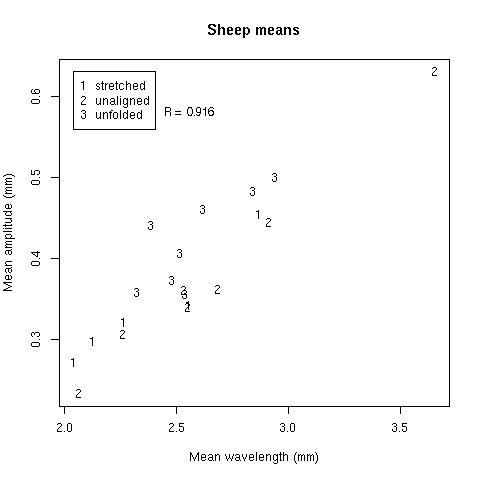
\includegraphics[width=1.0\textwidth]{figsfsheepmeans.png}
%   sheepmeanswa.png is original 
  \caption{Correlation between sheep means for Wavelength and Amplitude with CrimpType identified for each sheep. Means are averages over 15 fibres per sheep and 30 waves per fibre.}
  \label{fig:sfsheepmeans}
\end{figure}

%\end{document}


This is one way of checking whether CrimpType affects the relationship. What we see is a correlation of 0.916 which is computed ignoring crimptype. The unfolded crimptype is seen to have a slightly higer amplitude for a given wavelength than the other crimptypes. The correlation differs from the value of 0.974 calculated from variance components in the prevcious section for two reasons
\begin{itemize}
\item each mean plotted in Figure~\ref{fig:sfsheepmeans} is a mean of a finite number of observations so is subject to error. The correlation calculated from variance components is what the correlation in Figure~\ref{fig:sfsheepmeans} would be if there were a very large number of observations per sheep.
\item The correlation calculated from variance components is calculated from the SheepNo within Crimptype component - ie it is within crimptype and the difference in amplitude of the unfolded crimptype data noted above does not 'degrade' the correlation. In Figure~\ref{fig:sfsheepmeans} the differences in means between crimptypes do enter into the correlation.
\end{itemize}
Despite all that, we can still say that Figure~\ref{fig:sfsheepmeans} confirms the very high between sheep correlation of wavelength with amplitude. There is a suggestion in Figure~\ref{fig:sfsheepmeans} that the unfolded wools do not have quite as higha correlation as the other types. So if we use our crimp model (Jackson and Watts(2016)~\cite{jack:16}) at the sheep level we have to note that whatever determines wavelength also determines amplitude and it would be difficult to separate the two. It would be feasible, for example, if using our crimp model to predict sheep means, to measure only wavelength, and to obtain amplitude from wavelength using a regression equation. We fitted this regression at the level of sheep means, and obtained
\begin{displaymath}
amplitude = -0.2047  + crimptype deviation + 0.2305 * wavelength
\end{displaymath}
where the crimptype deviations are -0.0046 for stretched, -0.0274 for unaligned, and +0.0320 for unfolded. 
This allows for the slightly higher amplitudes of the unfolded crimptype seen in Figure~\ref{fig:sfsheepmeans}, but it does not allow for the possibility that wavelength and amplitude are less highly correlated at the sheep means level than the other types.

We will now have a look at the relationship between fibre means for wavelength and amplitude. In Figure~\ref{fig:sffibremeans} we plot the means for all $21 * 15 = 315$ fibres, this time ignoring both CrimpType and SheepNo.
%\documentclass{article}
%\usepackage{graphicx,subfigure}
%\begin{document}

\begin{figure}[!h]
  \centering
  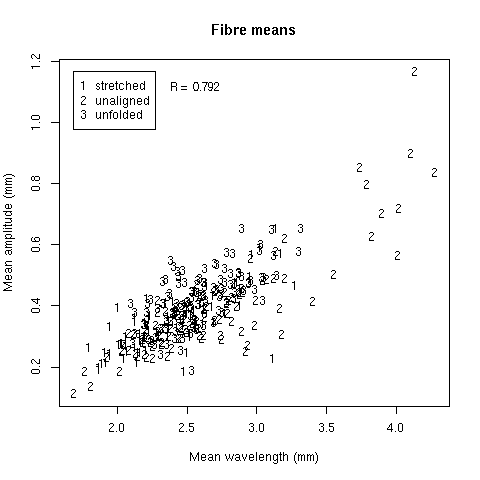
\includegraphics[width=1.0\textwidth]{figsffibremeans.png}
%   fibremeanswa.png is original 
  \caption{Correlation between fibre means for Wavelength and Amplitude with CrimpType identified for each fibre. Means are averages over 30 waves per fibre.}
  \label{fig:sffibremeans}
\end{figure}

%\end{document}


We see a correlation of 0.792 and this compares with the correlation of 0.667 obtained from variance components for the FibreNo within SheepNo within CrimpType effect.  The reasons for the difference are the same as given above for the between SheepNo correlation. It would seem that the variation between sheep means is contributing to the correlation observed in Figure~\ref{fig:sffibremeans} and is increasing it.

What we can do to try to more correctly visualize the between fibre within sheep correlation is to just looka at the correlation of fibre means for one sheep. This is done for SheepNo 1 in Figure~\ref{fig:sffibremeanssheep1}
%\documentclass{article}
%\usepackage{graphicx,subfigure}
%\begin{document}

\begin{figure}[!h]
  \centering
  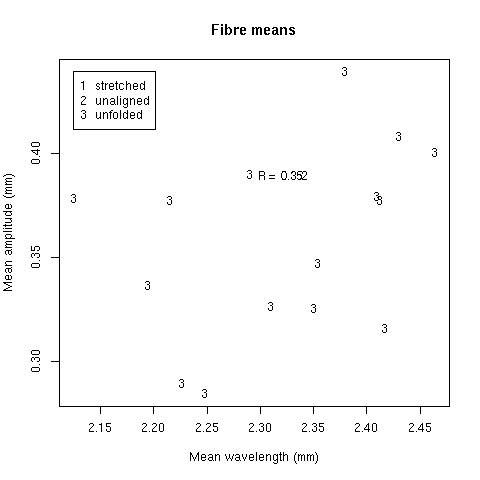
\includegraphics[width=1.0\textwidth]{figsffibremeanssheep1.png}
%   fibremeanswa.sheep1.png is original 
  \caption{Correlation between fibre means for Wavelength and Amplitude for SheepNo 1 only. Means are averages over 30 waves per fibre.}
  \label{fig:sffibremeanssheep1}
\end{figure}

%\end{document}


What we see is a correlation of 0.352 with a much reduced range of variation for both wavlength and amplitude.This is lower than the correlation of 0.667 obtained from variance components, but of course we have only looked at one sheep. 

We can conclude that there is a lower correlation between wavelength and amplitude at the fibre level than at the sheep level. So if we use our crimp model at the fibre level there is plenty of room for independent variation of wavelength and amplitude. A correlation of 0.7, for example, only means that half of the variance is in common.

Finally we want to look at the between waves within fibre correlation. The best we can do here is to simply plot all $21 * 15 * 30 = 9450$ wave measurements, ignoring CrimpType, SheepNo, and FibreNo. This is shown in Figure~\ref{fig:sfwavemeas}.
%\documentclass{article}
%\usepackage{graphicx,subfigure}
%\begin{document}

\begin{figure}[!h]
  \centering
  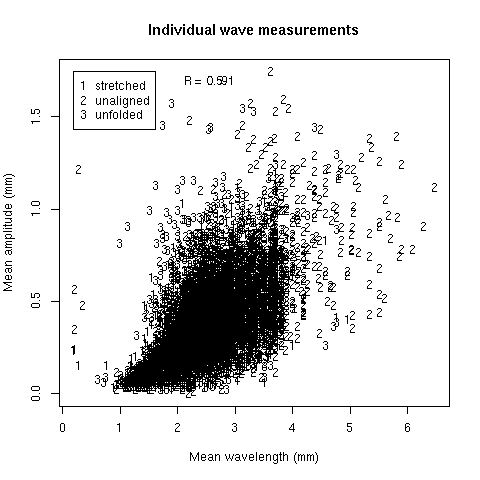
\includegraphics[width=1.0\textwidth]{figsfwavemeas.png}
%   wavemeaswa.png is original 
  \caption{Correlation between individual wave measurements for Wavelength and Amplitude with CrimpType identified for each fibre. }
  \label{fig:sfwavemeas}
\end{figure}

%\end{document}


We see a very crowded plot with a correlation of 0.591. Compare this with the correlation of 0.478 obtained for waves within fibre within sheep using variance components. The same comments apply as above. The differences between sheep and fibres have inflated the observed correlation.

We can conclude that there is an even lower correlation between wavelength and amplitude at the wave within fibre level. So if we use our crimp model on individual waves, there is almost independent variation of wavelength and amplitude. A correlation  of 0.5, for example, only means that 25 percent of the variation is in common.

Why should there be different correlations at different levels? Basically it is because the things causing wavelength and amplitude to vary at each level are different. At the sheep level the correlation of wavelength with amplitude is caused either by sheep differences in genes affecting both traits, or by sheep differences in environmental factors affecting both traits. At the fibre level within a sheep, the correlation is caused by whatever factors cause all wool follicles on a sheep to grow similar or dissimilar fibres, in this case, similar in both wavelength and amplitude. At the level of individual waves within a fibre, the correlation is caused by whatever controls variation in successive waves grown by a single follicle. This would include factors affecting what happens to the fibre in the staple after it is extruded from the follicle.

So the last word is - be careful about levels when looking at correlations. 


\clearpage
\section{Assessing measurement techniques by comparison of measured amplitude with OFDA fibre curvature measurements}
For each sheep, we have one measurement of mean fibre curvature ( degrees per mm) obtained with the OFDA 2000 instrument using the whole staple scanning technique.  This measurement can be converted to radius of curvature as follows
\begin{itemize}
\item change the OFDA curvature ( degrees per mm) to curvature in radians per mm using $C_{rads} = \pi C_{deg} / 180$
\item change from curvature to radius in mm using $R = 1/C_{rads}$
\end{itemize}
Note that radius of curvature measured this way ( in the staple) is not exactly intrinsic radius of curvature, because the fibres have a crimp {\em set} . So we have to take care relating OFDA radius to our amplitude measures. 


Figure~\ref{fig:ofdaradsfampl} show the sheep mean measured amplitude by our SF technique plotted against the OFDA radius of curvature.
%\documentclass{article}
%\usepackage{graphicx,subfigure}
%\begin{document}

\begin{figure}[!h]
  \centering
  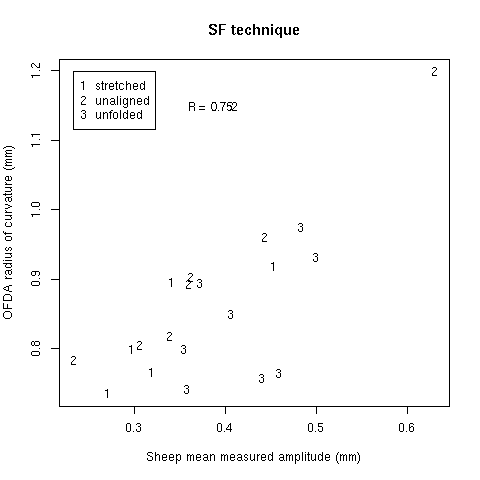
\includegraphics[width=1.0\textwidth]{figofdaradsfampl.png}
%   ofdaradsfampl.png is original 
  \caption{Correlation between sheep means for Amplitude measured by the SF technique and radius of curvature measured by OFDA staple scanning technique. CrimpType identified for each sheep. Means are averages over 30 waves per fibre.}
  \label{fig:ofdaradsfampl}
\end{figure}

%\end{document}


 The agreement is disasterously bad - the OFDA values are more than twice our measured amplitudes. The unfolded crimp type wools are different from the others in that OFDA measures a lower radius, but still not low enough to agree with our amplitudes. The correlation of 0.75 is not as strong as one would expect.

Given this poor result for the SF technique, there is no point, at this stage, in looking at the relationship for the IS annd FC techniques, as they measured smaller wavelengths than the SF technique for stretched and unaligned wools, and slightly larger wavelengths for unfolded wools. Their agreement with OFDA radius would be worse.

What we need to do first is to resolve the disagreement in Figure~\ref{fig:ofdaradsfampl}. We start by separating the unfolded wools from wools with a stretched helix crimp.

\subsection{Wools with a stretched or unaligned crimptype}
 Figure~\ref{fig:ofdaradsfamplhelix} shows  the same plot of SF technique amplitude against OFDA radius as Figure~\ref{fig:ofdaradsfampl}, just for the wools with stretched helix crimp ( stretched and unaligned).
%\documentclass{article}
%\usepackage{graphicx,subfigure}
%\begin{document}

\begin{figure}[!h]
  \centering
  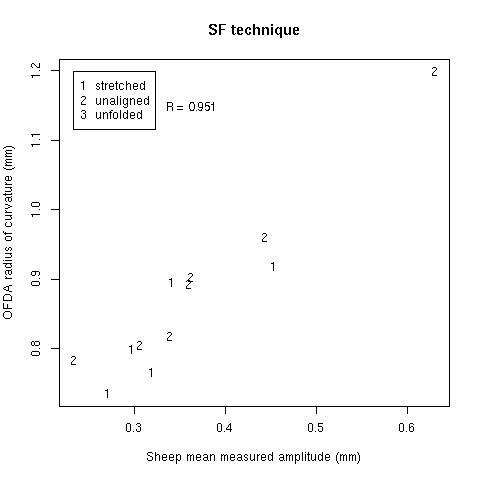
\includegraphics[width=1.0\textwidth]{figofdaradsfamplhelix.png}
%   ofdaradsfamplhelix.png is original 
  \caption{Correlation between sheep means for Amplitude measured by the SF technique and radius of curvature measured by OFDA staple scanning technique. CrimpTypes stretched and unaligned only. Means are averages over 30 waves per fibre.}
  \label{fig:ofdaradsfamplhelix}
\end{figure}

%\end{document}


What we have now is an excellent correlation of 0.951, so OFDA radius and SF amplitude both rank sheep in the same order. But we still have the disasterous difference in means with OFDA radius being more than twice our SF measured amplitude.

The radius of a stretched helix {\em is} its observed amplitude. So for a stretched helix crimp type, if OFDA measures the fibre curvature properly, the OFDA radius of curvature ($R$) should be equal to amplitude of the crimp wave in the staple ($a_{s}$) as measured by our three techniques ( IS,FC and SF). That is not happening, so, we have to think about what OFDA 2000 does in measuring curvature directly on staples.  Each stretched helix crimp is a 3 dimensional dished sine wave, but when viewed thru a microscope it would be seen as a planar image, that is as an ordinary 2 dimensional sine wave. While the radius of a stretched helix will be similar all along its length, and thus is of almost constant curvature, the curvature of a 2 dimensional sine wave varies along its length. A sine wave has maximum curvature at its peaks and troughs, and zero curvature at its points of inflection. So if OFDA measures curvature on a planar sine wave image, it measures something that varies along the length of the fibre image.  In this case, OFDA measured curvatures would vary from a maximum exceeding the 'true' 3 dimensional curvature at peaks and troughs, down to zero curvature at points of inflection.


Our SF technique uses a microscope too. Why would it not be subject to the same planar image problem? Because we measure amplitude, rather than curvature, and amplitude will be the same in the 2 dimensional planar image as it is in the 3 dimensional stretched helix.

To get 'true' curvature from an OFDA mean reading, we need to know the distribution of curvatures along a sine wave. If anyone wants to derive this theoretically they are welcome.  
 What we can do easily here is compute a simulated distribution of curvatures at all points along a planar sine wave. 
For any function $y = f(x)$, the curvature of the function line at all $x$ values is given by
\begin{equation}
\label{eqn:curv}
\kappa = \frac{ \frac{d^{2}y}{dx^{2}} } {[1 + (\frac{dy}{dx})^{2}]^{\frac{3}{2}}}
\end{equation}
So for the sine wave $y = a \sin{\theta}$ the derivatives are
\begin{eqnarray*}
\frac{dy}{d\theta} & = & a \cos{\theta} \\
\frac{d^{2}y}{d\theta^{2}} & = & -a \sin{\theta}
\end{eqnarray*}
However these derivatives are with respect to $\theta$.  What we need is derivatives with respect to $x$, where $x$ is distance along the X-axis of the sine wave plot. We note that as $\theta$ varies from $0$ to $ 2\pi$ , $x$ varies from $0$ to $\lambda$, where $\lambda$ is the wavelength. So we have the relation $\theta = \frac{2 \pi}{\lambda}$. This leads to the derivatiives 
\begin{eqnarray*}
\frac{dy}{dx} & = & \left(\frac{2 \pi}{\lambda}\right) a \cos{\left(\left(\frac{2 \pi}{\lambda}\right) x \right) } \\
\frac{d^{2}y}{dx^{2}} & = & -\left(\frac{2 \pi}{\lambda}\right)^{2} a  \sin{\left(\left(\frac{2 \pi}{\lambda}\right) x \right) }
\end{eqnarray*}

and the curvature (on the graph of $y$ against $x$ rather than $\theta$) is given by
\begin{equation}
\kappa = \frac{-\left(\frac{2 \pi}{\lambda}\right)^{2} a  \sin{\left(\left(\frac{2 \pi}{\lambda}\right) x \right) }}{[1 + (\left(\frac{2 \pi}{\lambda}\right) a \cos{\left(\left(\frac{2 \pi}{\lambda}\right) x\right) })^{2}]^{\frac{3}{2}}}
\end{equation}
This is obtained by substituting the derivatives with respect to $x$ into equation~\ref{eqn:curv}.
Note that wavelength ($\lambda$) enters into the formula for curvature as well as amplitude ($a$). This is because wavelength determines how obliquely OFDA views the curvature in a 2 dimensional image.

We plot $\kappa$ for $x= 0,\lambda$ mm  , an amplitude of $0.4$ mm and a wavelength of $2.2$ mm, in Figure~\ref{fig:sincurv}.
%\documentclass{article}
%\usepackage{graphicx,subfigure}
%\begin{document}

\begin{figure}[!h]
  \centering
  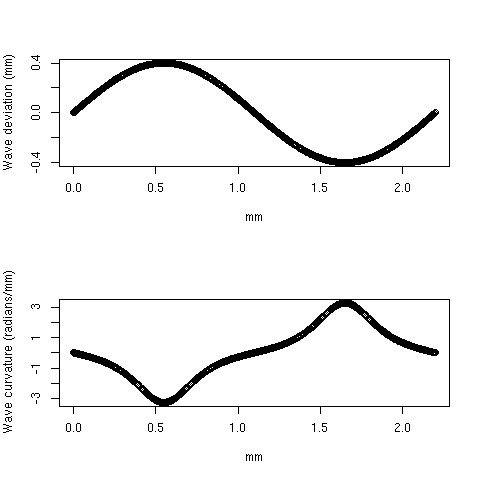
\includegraphics[width=1.0\textwidth]{figsincurv.png}
%   sincurv.png is original 
  \caption{Curvature at all points along a planar sine wave. The upper graph shows the sine wave for an amplitude of $0.4$ mm. The lower graph shows the corresponding curvatures in radians per mm}
  \label{fig:sincurv}
\end{figure}

%\end{document}


We see that curvatures are greatest at the peak and trough and zero at the inflection points. We also note that curvature is negative for curves where the concave side faces down, and positive for curves concave up. This is because we have calculated extrinsic curvature, relative to a set of axes. We can ignore sign for our purposes since OFDA measures intrinsic curvature, which is curvature ignoring any axes external to the object. (Note: the term 'intrinsic' here has nothing to do with the term 'intrinsic fibre curvature' used elsewhere in this document)

What we need to do now is simulate a sampling distribution of a set of curvatures sampled from points taken at random along the sine wave.  To do this we generated 5000 points sampled from the range $0$ to $2\pi$ for $\theta$ being the angle in the equation $y = a \sin{\theta}$. This ensures an equal probability of sampling at any point along the sine curve.  We then calculated the absolute value of curvature at each point $x = \left(\frac{\lambda}{2\pi}\right)\theta$ assuming an amplitude of 0.4 mm and a wavelength of 2.2 mm, and drew the histogram of curvatures.  The resultant histogram is shown in Figure~\ref{fig:curvhist}.
%\documentclass{article}
%\usepackage{graphicx,subfigure}
%\begin{document}

\begin{figure}[!h]
  \centering
  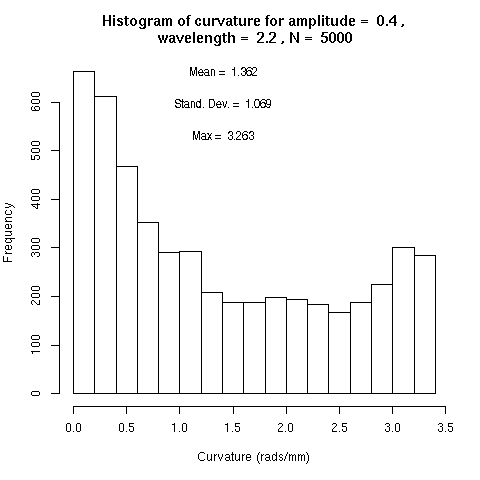
\includegraphics[width=1.0\textwidth]{figcurvhist.png}
%   curvhist.png is original 
  \caption{Simulated histogram of intrinsic curvatures at 5000 points sampled at random along a sine wave of amplitude 0.4 mm over the interval 0 to $2 * \pi$ radians. Curvatures in radians per mm. Mean and standard deviation calculated from histogram data.}
  \label{fig:curvhist}
\end{figure}

%\end{document}


What we see is a range of values of curvature from zero to 3.26, and the distribution is far from uniform, having a peaks at zero and 3.26 rads per mm. The reciprocal of this maximum value ($1/3.26 = 0.307$) is less than the nominal amplitude ($0.4$ mm). That is because the fibre is seen obliquely in the planar image.
The actual relation between maximum curvature of the planar sine wave ($\kappa_{max}$)(rads per mm) and the radius of the generating stretched helix ($a$)(mm) is
\begin{displaymath}
a = \left(\frac{\lambda}{2 \pi}\right)^{2} \kappa_{max}
\end{displaymath}
For example, for the case in Figure~\ref{fig:curvhist} $\left(\frac{\lambda}{2 \pi}\right)^{2} = 0.1227$, so $a = (.1227)(3.26) = 0.40$, which is correct as we started with an amplitude of $0.4$. 

Wavelength is present in the above formula because it determines how obliquely the planar view sees the fibre curvature. The ratio $\frac{\lambda}{2 \pi}$ is the pitch per radian of the stretched helix - ie how far the crimp wave moves in the X direction with 1 radian of rotation around the helix circle. 

This shows that we can  not expect a planar mean curvature measurement, such as reported by OFDA,  to agree with the helix radius or amplitude. We need the maximum planar curvature to derive helix radius or amplitude, and OFDA does not report maximum planar curvature. We cannot derive the maximum planar curvature from the mean planar curvature and its standard deviation, because we do not know the form of the distribution of planar curvatures, we only have a simulation.
 For example, the reciprocal of the mean planar curvature from our simulation example in Figure~\ref{fig:curvhist}, $1/1.0686 = 0.9358$ gives a radius (mm) much greater than the known amplitude of 0.4. 

 OFDA reports mean curvature ($\kappa_{mean}$) and standard deviation of curvatures ($\kappa_{sd}$). It does not report maximum curvature ($\kappa_{max}$), so we cannot convert OFDA results back to amplitude ($a$) or helix radius. We can, however, forward convert our amplitude and wavelength measurements to $\kappa_{max}$, $\kappa_{mean}$, and $\kappa_{sd}$, using the above simulation calculation. We did this for the 12 sheep with stretched helix crimp ( ie stretched and unaligned crimp types) from our set of 21 sheep measured by our three techniques (SF,IS,FC) for ampltude and wavelength. For the SF technique the results are listed in Table~\ref{tab:ofdasimsf}.
%\documentclass{article}
%\usepackage{lscape}
%\begin{document}

\begin{table}[htp]
\centering
\caption{Measured amplitude and wavelength, by the SF technique, converted to simulated values of $\kappa_{mean}$, $\kappa_{sd}$, and $\kappa_{max}$ for 12 sheep with stretched helix crimp form. Comparison with OFDA mean curvature and standard deviation of curvature.}
\label{tab:ofdasimsf}
\vspace{0.1in}
\begin{tabular}{|p{0.4in}|p{0.4in}|p{0.4in}|p{0.6in}|p{0.6in}|p{0.5in}|p{0.5in}|p{0.6in}|} \hline
  Sheep No &   Wave length  & Ampl itude & Simulated $\kappa_{max}$  & Simulated $\kappa_{mean}$ & Simulated $\kappa_{sd}$ & OFDA mean curvature & OFDA stand. dev. curvature  \\  \hline
  14416 & 2.91  & 0.444  & 2.0699 & 0.9609 & 0.6775 & 1.041 & 0.7347  \\ 
  14498 & 2.87  & 0.454  & 2.1910 & 0.9931 & 0.7132 & 1.089 & 0.7836  \\
  14499 & 2.55  & 0.342  & 2.0763 & 1.0059 & 0.6708 & 1.117 & 0.8604  \\
  14516 & 2.53  & 0.360  & 2.2203 & 1.0522 & 0.7176 & 1.121 & 0.8046  \\ 
  14530 & 2.06  & 0.234  & 2.1676 & 1.1114 & 0.7011 & 1.278 & 0.8744  \\
  14544 & 2.27  & 0.320  & 2.4733 & 1.1910 & 0.8015 & 1.307 & 0.9337  \\
  14549 & 2.55  & 0.340  & 2.0581 & 1.0042 & 0.6669 & 1.223 & 0.8709  \\ 
  14564 & 2.26  & 0.306  & 2.3651 & 1.1518 & 0.7689 & 1.243 & 0.9076  \\
  14570 & 2.04  & 0.271  & 2.5961 & 1.2756 & 0.8381 & 1.360 & 0.9111  \\
  14574 & 2.13  & 0.297  & 2.6088 & 1.2386 & 0.8493 & 1.251 & 0.9093  \\ 
  14584 & 3.67  & 0.631  & 1.8668 & 0.8092 & 0.6157 & 0.834 & 0.6720  \\
  14592 & 2.68  & 0.362  & 1.9897 & 0.9743 & 0.6532 & 1.108 & 0.9041  \\ \hline
\end{tabular}
\end{table}

%\end{document}

The simulated $\kappa_{mean}$ values are quite close to the OFDA reported mean curvatures. This encourages us to think that
\begin{itemize}
\item our proposition that OFDA measures mean planar curvature is correct
\item our OFDA simulation based on a planar sine wave is correct
\item we may be able to use the simulated values of $\kappa_{mean}$ to assess our SF,IS, ans FC measuring techniques, assuming that best agreement with OFDA mean curvature implies best measuring technique.
\end{itemize} 


 For the SF technique, we plot $\kappa_{mean}$ against OFDA mean curvature in Figure~\ref{fig:ofdasimsfmean}.
%\documentclass{article}
%\usepackage{graphicx,subfigure}
%\begin{document}

\begin{figure}[!h]
  \centering
  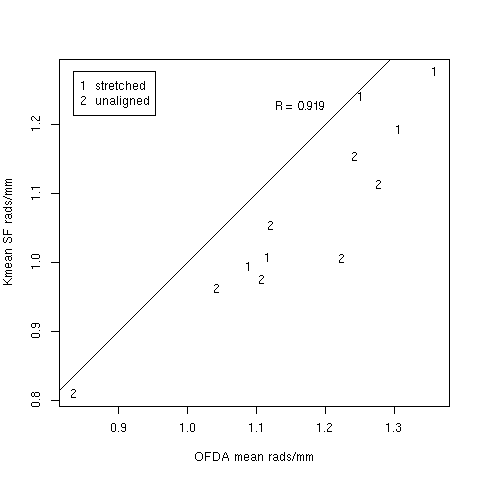
\includegraphics[width=1.0\textwidth]{figofdasimsfmean.png}
%   ofda.sf.stretch.mean.png is original 
  \caption{Simulation of OFDA results from measurements of wavelength and amplitude by the SF technique. Plot of $\kappa_{mean}$ against OFDA mean curvature. Solid line represents a one-to-one relationship.}
\label{fig:ofdasimsfmean}
\end{figure}

%\end{document}


We get a correlation of 0.92 between $\kappa_{mean}$ and OFDA mean curvature, and there is a slight bias with OFDA mean curvature being larger by about 0.1 rads per mm.  The bias may be due to bias in the measured wavelength and amplitude.

 Again for the SF technique, we plot $\kappa_{sd}$ against OFDA standard deviation of curvature in Figure~\ref{fig:ofdasimsfsd}.
%\documentclass{article}
%\usepackage{graphicx,subfigure}
%\begin{document}

\begin{figure}[!h]
  \centering
  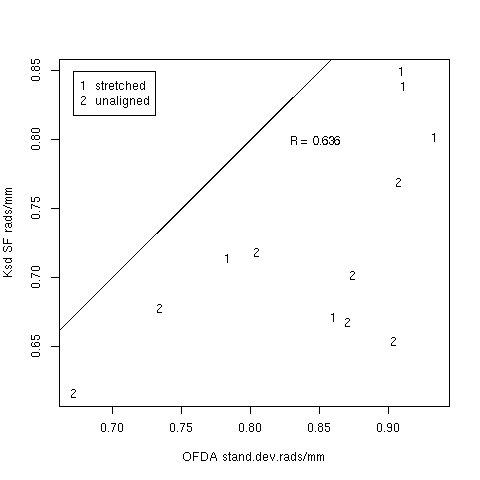
\includegraphics[width=1.0\textwidth]{figofdasimsfsd.png}
%   ofda.sf.stretch.sd.png is original 
  \caption{Simulation of OFDA results from measurements of wavelength and amplitude by the SF technique. Plot of $\kappa_{sd}$ against OFDA standard deviation of curvature. Solid line represents a one-to-one relationship.}
\label{fig:ofdasimsfsd}
\end{figure}

%\end{document}


For the standard deviation we get a poorer correlation and a large bias, OFDA standard deviation of curvature being much larger than our simulation. This is not unexpected. Our simulation only calculates the standard deviation due to variations in curvature along a planar sine wave of given wavelength and amplitude. It does not include variation in wavelength and amplitude along the fibre or between fibres, and we know from Section~\ref{sf2010} that these sources of variation are significant. OFDA measures what is 'sees' so includes all sources of variation, so its standard deviation is larger.

For the FC and IS techniques , we plot $\kappa_{mean}$ against OFDA mean curvature in Figures~\ref{fig:ofdasimfcmean} and \ref{fig:ofdasimismean}.
%\documentclass{article}
%\usepackage{graphicx,subfigure}
%\begin{document}

\begin{figure}[!h]
  \centering
  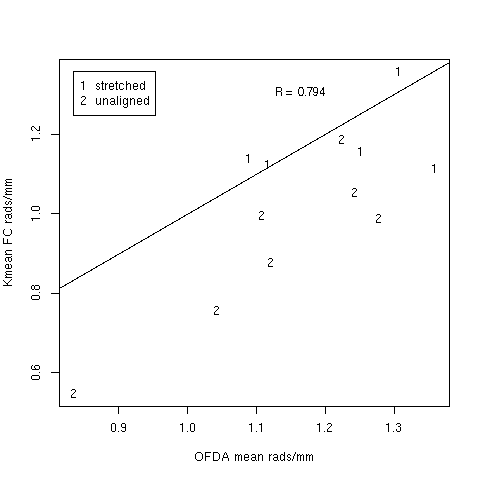
\includegraphics[width=1.0\textwidth]{figofdasimfcmean.png}
%   ofda.fc.stretch.mean.png is original 
  \caption{Simulation of OFDA results from measurements of wavelength and amplitude by the FC technique. Plot of $\kappa_{mean}$ against OFDA mean curvature. Solid line represents a one-to-one relationship.}
\label{fig:ofdasimfcmean}
\end{figure}

%\end{document}


%\documentclass{article}
%\usepackage{graphicx,subfigure}
%\begin{document}

\begin{figure}[!h]
  \centering
  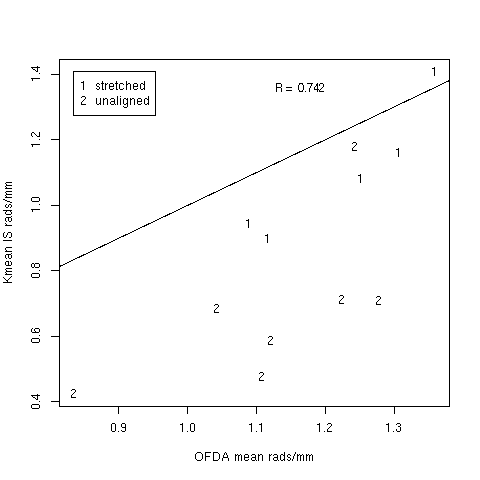
\includegraphics[width=1.0\textwidth]{figofdasimismean.png}
%   ofda.is.stretch.mean.png is original 
  \caption{Simulation of OFDA results from measurements of wavelength and amplitude by the IS technique. Plot of $\kappa_{mean}$ against OFDA mean curvature. Solid line represents a one-to-one relationship.}
\label{fig:ofdasimismean}
\end{figure}

%\end{document}


For the FC technique (Figure~\ref{fig:ofdasimfcmean}) we get a correlation of 0.79, and a slightly greater bias than for SF technique. For the IS technique we get a correlation of 0.74, and a quite large bias, OFDA mean being about 0.4 rads per mm larger than our simulated mean from  the IS measurements of wavelength and amplitude. 

So here we have our first instance of an external criterion which could tell us which of the three techniques ( SF,FC,IS ) for wavelength and amplitude measurement is least biased. The indication seems to be that the SF technique is the least biased.  Wavelength and amplitude measured by the SF technique lead to a simulated $\kappa_{mean}$ which is not very different from the OFDA measured mean curvature. We should note that this is a test of wavelength and amplitude measurements jointly. It is not possible to separate them as they are both used in simulation of $\kappa_{mean}$. Remember also that wavelength and amplitude are very highly correlated at the sheep means level.

There remains one further question. We know from Figures~\ref{fig:unfold}, \ref{fig:stretch}, and ~\ref{fig:unalign} that wavelength varies along the 30 successive waves measured by the SF technique on each fibre, there being a decline in wavelength from base to tip end of the fibre, while amplitude exhibits a very slight decline for stretched and unaligned wools, and the opposite for unfolded wools. One has to ask whether there is a change in the simulated $\kappa_{mean}$ value along the fibre, and whether there is a most favourable wave position at which to take the measurement?

We tackle this question by dividing the succesive wave measurements from the SF technique into 
\begin{description}
\item[base] first 10 wave positions starting from the staple base
\item[mid] next 10 wave positions after base
\item[tip] last 10 wave positions ending at the staple tip
\end{description} 
We now compute the mean amplitude and wavelength for base, mid and tip regions, and use these to calculate the siimulated $\kappa_{mean}$ for each of base, mid, and tip, and then plot each of these against OFDA measured mean curvature. These three plots are shown in Figures~\ref{fig:ofdasimsfbasemean}, \ref{fig:ofdasimsfmidmean} and \ref{fig:ofdasimsftipmean}.
%\documentclass{article}
%\usepackage{graphicx,subfigure}
%\begin{document}

\begin{figure}[!h]
  \centering
  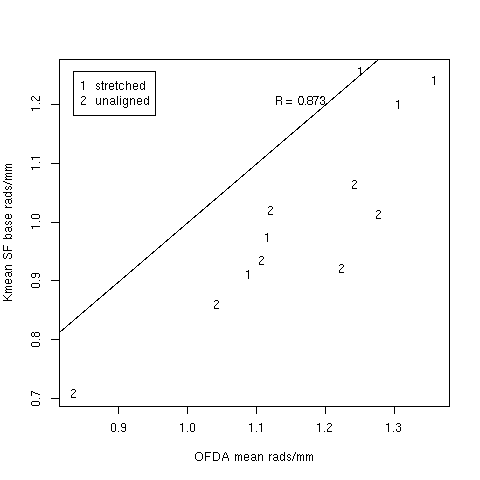
\includegraphics[width=1.0\textwidth]{figofdasimsfbasemean.png}
%   ofda.sfbase.stretch.mean.png is original 
  \caption{Simulation of OFDA results from measurements of wavelength and amplitude of the base region by the SF technique. Plot of $\kappa_{mean}$ against OFDA mean curvature. Solid line represents a one-to-one relationship.}
\label{fig:ofdasimsfbasemean}
\end{figure}

%\end{document}


%\documentclass{article}
%\usepackage{graphicx,subfigure}
%\begin{document}

\begin{figure}[!h]
  \centering
  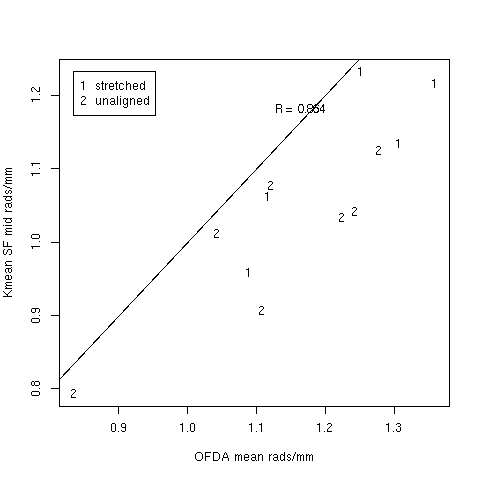
\includegraphics[width=1.0\textwidth]{figofdasimsfmidmean.png}
%   ofda.sfmid.stretch.mean.png is original 
  \caption{Simulation of OFDA results from measurements of wavelength and amplitude of the mid region by the SF technique. Plot of $\kappa_{mean}$ against OFDA mean curvature. Solid line represents a one-to-one relationship.}
\label{fig:ofdasimsfmidmean}
\end{figure}

%\end{document}


%\documentclass{article}
%\usepackage{graphicx,subfigure}
%\begin{document}

\begin{figure}[!h]
  \centering
  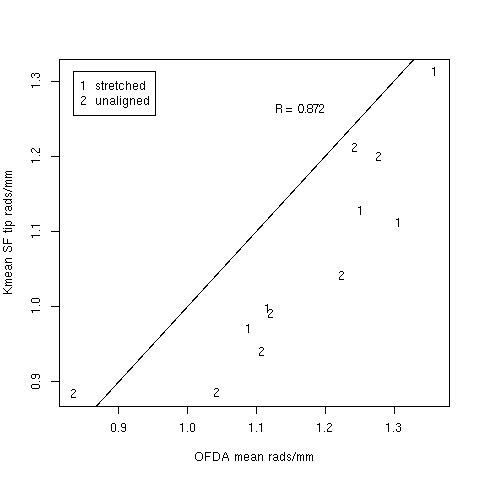
\includegraphics[width=1.0\textwidth]{figofdasimsftipmean.png}
%   ofda.sftip.stretch.mean.png is original 
  \caption{Simulation of OFDA results from measurements of wavelength and amplitude of the tip region by the SF technique. Plot of $\kappa_{mean}$ against OFDA mean curvature. Solid line represents a one-to-one relationship.}
\label{fig:ofdasimsftipmean}
\end{figure}

%\end{document}


What we see is that the correlation of $\kappa_{mean}$ with OFDA measured curvature is almost the same for all three regions, but is lower than the correlation obtained in Figure~\ref{fig:ofdasimsfmean} using data for all three regions pooled This is not surprising, the pooled data would have more accurate amplitude and wavelength measurements. For all three regions there is still a bias with our simulated $\kappa_{mean}$ being less then OFDA measured curvature. The bias is not the same for all three regions, the base region has a bias of about 0.2, and the other two regions have a bias of about 0.1 rads per mm.

So we have to conclude that there is something peculiar about the base region measurements of wavelength and amplitude by the SF technique which cause the bias relative to OFDA to be increased. Possible reasons for this are
\begin{itemize}
\item the procedure for removing the fibre from the staple for measurement distorted the crimp waves at the base. It may have also distorted the crimp waves of the other regions but not as much.
\item the fibre is held under some tension in the staple structure, and when the fibre is removed from the staple these constraints disappear and the crimp waves change. 
\end{itemize}

We know that the crimp waves elongate when a fibre is removed from a staple because the measured length of the removed fibre in a relaxed state ( ie not under tension) is larger than the staple length. This is shown in Figure~\ref{fig:LrLs} which plots relaxed fibre length against staple length.
%\documentclass{article}
%\usepackage{graphicx,subfigure}
%\begin{document}

\begin{figure}[!h]
  \centering
  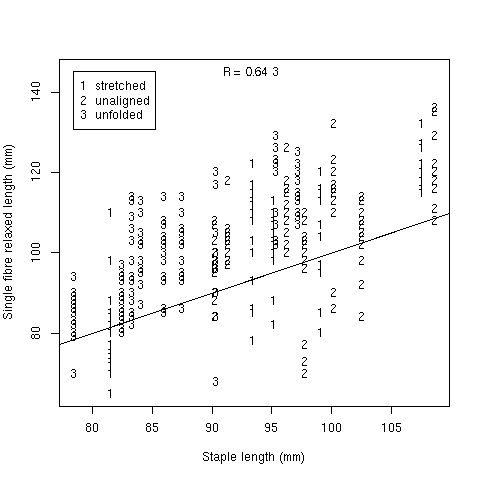
\includegraphics[width=1.0\textwidth]{figLrLs.png}
%   15fibreLsLr.png is original 
  \caption{Plot of staple length against relaxed fibre length for fibres removed from staples for the SF technique. There are 15 fibres per sheep, one staple per sheep, and 21 sheep}
\label{fig:LrLs}
\end{figure}

%\end{document}


We see that most of the fibres from each staple appear above the one-to-one line and therefore have relaxed lengths longer than the staple, the difference being about 10 mm. It might appear from Figure~\ref{fig:LrLs} that the unfolded wools have a larger difference between relaxed fibre length and staple length. That is correct, but all crimptypes exhibit this effect, as is shown in the boxplot of Figure~\ref{fig:LrminusLs}.
%\documentclass{article}
%\usepackage{graphicx,subfigure}
%\begin{document}

\begin{figure}[!h]
  \centering
  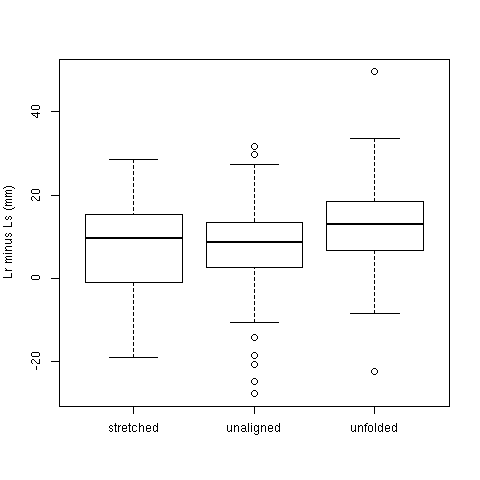
\includegraphics[width=1.0\textwidth]{figLrminusLs.png}
%   15fibreLrminusLs.png is original 
  \caption{Boxplot of relaxed fibre length minus staple length for fibres removed from staples for the SF technique, separately for each crimptype. There are 15 fibres per sheep, one staple per sheep and 21 sheep. The median values for each crimptype are stretched 9.56, unaligned 8.70, and unfolded 12.85.}
\label{fig:LrminusLs}
\end{figure}

%\end{document}


 This  must change the crimp amplitude and wavelength measurements relative to what they were undisturbed in the staple. It is something we have to put up with in order to use the SF technique which seems to be the 'best' technique, at least when assessed against OFDA mean curvature.

\clearpage
\subsection{Wools with an unfolded crimptype}
	We now need to do our assessment against OFDA mean curvature all over again for wools of unfolded crimptype. Figure~\ref{fig:ofdaradsfamplunfold}  shows the same plot of SF technique amplitude against OFDA radius as Figure~\ref{fig:ofdaradsfampl}, just for wools with an unfolded crimp.
%\documentclass{article}
%\usepackage{graphicx,subfigure}
%\begin{document}

\begin{figure}[!h]
  \centering
  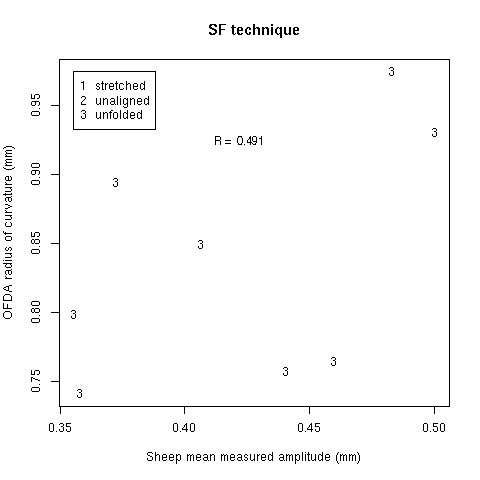
\includegraphics[width=1.0\textwidth]{figofdaradsfamplunfold.png}
%   ofdaradsfamplunfold.png is original 
  \caption{Correlation between sheep means for Amplitude measured by the SF technique and radius of curvature measured by OFDA staple scanning technique. CrimpType unfolded only. Means are averages over 30 waves per fibre.}
  \label{fig:ofdaradsfamplunfold}
\end{figure}

%\end{document}


We see a very poor correlation and a large bias with OFDA mean radius of curvature being about twice the amplitude measured by our SF technique.

We have to think about how OFDA would 'see' an unfolded crimp in the staple.
For an unfolded crimp type the OFDA radius of curvature ($R$) should be the intrinsic radius of curvature, if we ignore the regions of the semicircular crimp wave where the fibres are twisted. This is because, in an unfolded crimp wool, the crimp loops unfold without stretching, so the intrinsic radius of the fibre is preserved in the staple. The problem of OFDA using a planar image does not occur for unfolded wools, because successive loops unfold approximately 180 degrees in opposite directions so the crimp wave is close to flat, and a planar image sees it without distortion. 

So if OFDA curvature is OK for unfolded wools, we have to think about what our measured amplitude and wavelength mean.  The meaning of measured amplitude of an unfolded wool varies with the angle between unfoldings. Only in the case where the angle between unfoldings is exactly 180 degrees will the measured amplitude equal intrinsic radius. For unfoldings greater than 180 degrees amplitude will exceed intrinsic radius, and for unfoldings less than 180 degrees amplitude will be less than intrinsic radius. So in the unfolded wools case, we need to 'convert' our amplitude measurements to intrinsic radius, to be able to assess them against OFDA.

The way to 'convert' our amplitude measurements is to make use of our model for unfolded crimp (Jackson and Watts (2016)~\cite{jack:16} to calculate intrinsic radius ($a$) and angle between unfoldings ($\theta$) from measured wavelength and amplitude.  We do this for the eight unfolded wools shown in Figure~\ref{fig:ofdaradsfamplunfold} and the results are shown in Table~\ref{tab:waradthetaunfold}
%\documentclass{article}
%\usepackage{lscape}
%\begin{document}

\begin{table}[htp]
\centering
\caption{Measured amplitude and wavelength, by the SF technique, converted to values of intrinsic radius ($a$) and angle between unfoldings ($\theta$) for 8 sheep with unfolded helix crimp form. Comparison with OFDA mean curvature ($C$) converted to radius of curvature ($R$).}
\label{tab:waradthetaunfold}
\vspace{0.1in}
\begin{tabular}{|p{0.4in}|p{0.4in}|p{0.4in}|p{0.6in}|p{0.6in}|p{0.5in}|p{0.6in}|} \hline
  Sheep No &   Wave length  & Ampl itude & Intrinsic radius (mm)  & Angle between unfoldings (degrees) &  OFDA mean curvature (rads/mm) & OFDA radius of curvature (mm) \\  \hline
  14355 & 2.32  & 0.358  & 0.648 & 126.7  & 1.349 & 0.7412   \\ 
  14406 & 2.52  & 0.406  & 0.692 & 131.1 & 1.178 & 0.8488   \\
  14408 & 2.62  & 0.460  & 0.696 & 140.3 & 1.309 & 0.7639   \\
  14413 & 2.84  & 0.483  & 0.763 & 136.9 & 1.026 & 0.9744   \\ 
  14525 & 2.94  & 0.500  & 0.790 & 136.9 & 1.253 & 0.7980   \\
  14526 & 2.54  & 0.355  & 0.745 & 116.8 & 1.278 & 0.7827   \\
  14586 & 2.39  & 0.441  & 0.625 & 145.7 & 1.321 & 0.7569   \\ 
  14593 & 2.48  & 0.372  & 0.702 & 123.8 & 1.119 & 0.8938   \\ \hline
\end{tabular}
\end{table}

%\end{document}

We see that our intrinsic radius calculated from wavelength and amplitude measured by the SF technique, is of similar magnitude to the OFDA radius of curvature calculated from OFDA mean curvature measurements.  The reason the intrinsic radii are larger than the measured amplitudes in these data is that the angle between unfoldings for these wools is less than 180 degrees. If we now plot these data we get Figure~\ref{fig:waradthetaunfoldsf}
%\documentclass{article}
%\usepackage{graphicx,subfigure}
%\begin{document}

\begin{figure}[!h]
  \centering
  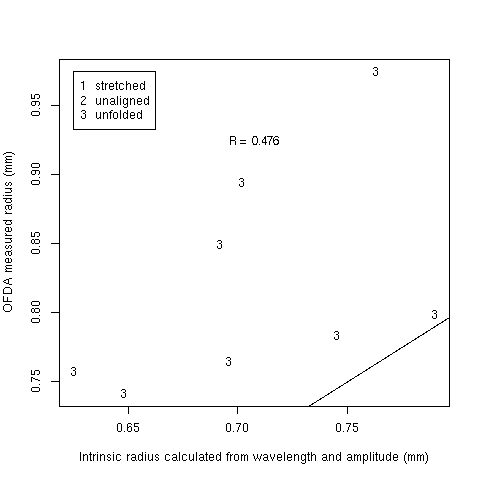
\includegraphics[width=1.0\textwidth]{figwaradthetaunfoldsf.png}
%   figwaradthetaunfoldsf.png is original 
  \caption{Intrinsic radius of curvature calculated from wavelength and amplitude measured by the SF technique, plotted against OFDA measured radius of curvature for unfolded wools only. Each point is a sheep mean.}
  \label{fig:waradthetaunfoldsf}
\end{figure}

%\end{document}


 The correlation is only increased slightly, and the OFDA radius measurement is still larger than the calculated intrinsic radius but only by about 0.1 mm. This is a much smaller bias than the 0.4 mm we started with in Figure~\ref{fig:ofdaradsfamplunfold}.
There are several possible explanations of this less than satisfactory result.
\begin{itemize}
\item  the unfolded crimp waves may not be perfectly flat ( ie unfolded 180 degrees). In this case OFDA would see each half wave as a part of an ellipse instead of as part of a circle. A circle viewed at an angle is an ellipse. Curvature of an elliptical fibre image varies around the ellipse, is least at the peaks of the wave, and should equal the circle's curvature near the inflection points. So the average curvature would be less, which means the radius of curvature would be larger. This is what we observe - OFDA radii are larger than intrinsic radii calculated from our own wavelength and amplitude measurements. We have no way of adjusting OFDA results for this, because we have no measure of the angle each loop unfolds to.
\item the calculation of intrinsic radius and angle between unfoldings from our wavelength and amplitude measurements is quite sensitive to the balance between wavelength and amplitude.  If our measurement technique gets the ratio of wavelength to amplitude wrong, the calculation of intrinsic radius will be wrong. We need to compare all three measurement techniques and see if one does a better job of getting the balance right.
\item there may be a scale problem here. The unfolded wools do not vary much in radius of curvature so their differences may be too small for the precision of our measurements. This would explain the poor correlation, but not the remaining bias in Figure~\ref{fig:waradthetaunfoldsf}.
\end{itemize}
The one thing we can do is look at the other (FC and IS) measurement techniques and check if the region measured ( tip,mid, or base) has any effect on results for the SF technique. 

For the FC and IS techniques the equivalent graphs to Figure~\ref{fig:waradthetaunfoldsf} are given in Figures~\ref{fig:waradthetaunfoldfc} and \ref{fig:waradthetaunfoldis}.
%\documentclass{article}
%\usepackage{graphicx,subfigure}
%\begin{document}

\begin{figure}[!h]
  \centering
  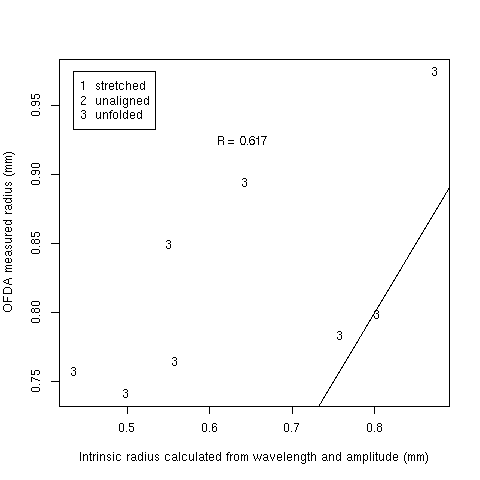
\includegraphics[width=1.0\textwidth]{figwaradthetaunfoldfc.png}
%   figwaradthetaunfoldfc.png is original 
  \caption{Intrinsic radius of curvature calculated from wavelength and amplitude measured by the FC technique, plotted against OFDA measured radius of curvature for unfolded wools only. Each point is a sheep mean.}
  \label{fig:waradthetaunfoldfc}
\end{figure}

%\end{document}


%\documentclass{article}
%\usepackage{graphicx,subfigure}
%\begin{document}

\begin{figure}[!h]
  \centering
  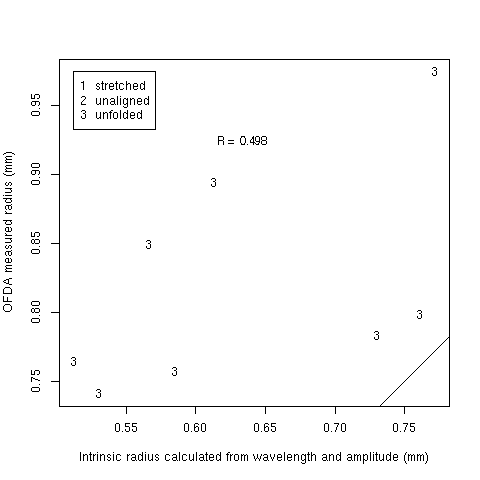
\includegraphics[width=1.0\textwidth]{figwaradthetaunfoldis.png}
%   figwaradthetaunfoldis.png is original 
  \caption{Intrinsic radius of curvature calculated from wavelength and amplitude measured by the IS technique, plotted against OFDA measured radius of curvature for unfolded wools only. Each point is a sheep mean.}
  \label{fig:waradthetaunfoldis}
\end{figure}

%\end{document}


We see that FC and IS both give a smaller calculated intrinsic radius than the OFDA measured radius, so they are similar to the SF technique in bias. The correlations are all poor. The three techniques basically agree on intrinsic radius. This can be seen if we cross-correlate the calculated intrinsic radii - for SF x FC r = .95, for SF x IS r = .83, and for FC x IS r = .91. This is not the case for calculated theta, however. The cross-correlations for calculated theta are for SF x FC r = .21, for SF x IS r = .07, and for FC x IS r = .84. Only for FC x IS is there a cross-technique repeatability for calculated theta. This suggests that SF is different in some way from the other two techniques. It may be useful therefore to look at regions (tip, mid, and base) separately for the SF technique.

For the SF technique, the graphs equivalent to Figure~\ref{fig:waradthetaunfoldsf} but with base, mid, and tip regions separated are given in Figures~\ref{fig:waradthetaunfoldsfbase}, \ref{fig:waradthetaunfoldsfmid}, and \ref{fig:waradthetaunfoldsftip}.
%\documentclass{article}
%\usepackage{graphicx,subfigure}
%\begin{document}

\begin{figure}[!h]
  \centering
  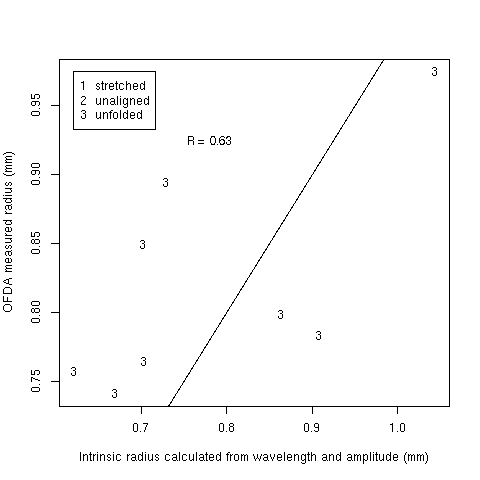
\includegraphics[width=1.0\textwidth]{figwaradthetaunfoldsfbase.png}
%   figwaradthetaunfoldsfbase.png is original 
  \caption{Intrinsic radius of curvature calculated from wavelength and amplitude measured by the SF technique on the base region of each staple, plotted against OFDA measured radius of curvature for unfolded wools only. Each point is a sheep mean for the base region.}
  \label{fig:waradthetaunfoldsfbase}
\end{figure}

%\end{document}


%\documentclass{article}
%\usepackage{graphicx,subfigure}
%\begin{document}

\begin{figure}[!h]
  \centering
  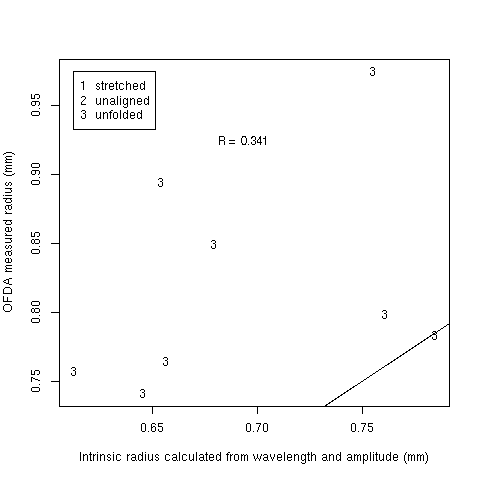
\includegraphics[width=1.0\textwidth]{figwaradthetaunfoldsfmid.png}
%   figwaradthetaunfoldsfmid.png is original 
  \caption{Intrinsic radius of curvature calculated from wavelength and amplitude measured by the SF technique on the middle region of each staple, plotted against OFDA measured radius of curvature for unfolded wools only. Each point is a sheep mean for the middle region.}
  \label{fig:waradthetaunfoldsfmid}
\end{figure}

%\end{document}


%\documentclass{article}
%\usepackage{graphicx,subfigure}
%\begin{document}

\begin{figure}[!h]
  \centering
  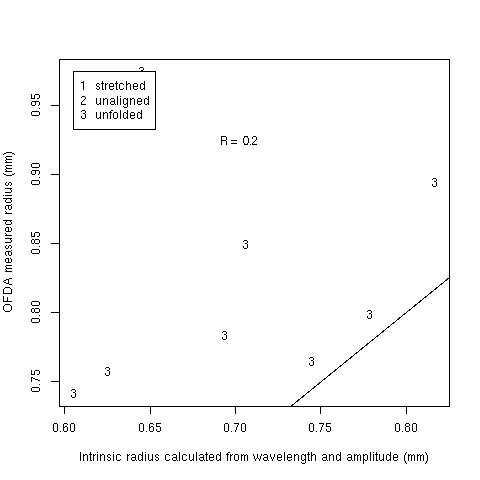
\includegraphics[width=1.0\textwidth]{figwaradthetaunfoldsftip.png}
%   figwaradthetaunfoldsftip.png is original 
  \caption{Intrinsic radius of curvature calculated from wavelength and amplitude measured by the SF technique on the tip region of each staple, plotted against OFDA measured radius of curvature for unfolded wools only. Each point is a sheep mean for the tip region.}
  \label{fig:waradthetaunfoldsftip}
\end{figure}

%\end{document}


We see that for the base region the correlation with OFDA measured radius is 0.63 and there is no obvious bias, while for the mid and tip regions the correlation with OFDA measured radius is very low and there is still a bias of about 0.1 mm withthe OFDA measured radius being larger.

 So we have just one satisfactory result for unfolded wools - if we use the SF technique on the base region to measurte wavelength and amplitude and then calculate intrinsic radius, it correlates well with OFDA measured radius and is unbiased.  All other approaches ( FC or IS or SF on mid or tip or whole staple) are poorly correlated with OFDA radius and are biased. We can interpret this in a number of ways
\begin{itemize}
\item perhaps OFDA only measures its curvature on the base region of staples. We do not know, OFDA methodology is a black box.
\item perhaps the FC and IS techniques are simply innacurate because of inadequate replication. However this did not seem to be the case with stretched helix wools.
\item remember that the base region had longer wavelengths than mid and tip. This might lead one to suspect that the process of removing the fibre from the staple used in the SF technique had extended the base region. But in that case how could the base region agree better with OFDA?
\item the opposite of the previous item. Perhaps the fibres in the mid and tip regions of the staple are compressed in some way so that the wavelengths are shorter. Then when the SF technique removes the fibre from the staple for measurement some, but not all, of the compression relaxes so that the wavelengths partially recover. This seems likely as it explains two phenomena - the relaxed length of the removed fibre being longer than the staple, and the better result for intrinsic radius calculation from wavelength and amplitude of the base region. 
\item remember that for unfolded wools the SF technique measured a lower amplitude at the base region compared to FC and IS, while for stretched helix wools SF measured a higher amplitude at the base region compared with FC and IS. This suggests that the fibre removal process in SF technique did something different to unfolded wools compared to stretched helix wools. 
\item remember that we are calculating intrinsic curvature from measured wavelength and amplitude. It may be that fibres in the tip and mid regions are more disturbed and therefore are a reflection of things additional to intrinsic curvature. But in that case why dont IS and FC techniques work as they are on the base region?
\end{itemize}

So we are left with a mystery result. We have to leave it stand, and see if other approached shed light on the above issues


\clearpage
\section{Assessing measurement techniques by comparison of measured wavelength with wavelength derived from crimp frequency measurement on a staple using a crimp meter}
We can compare each of our measurement techniques for wavelength, with wavelength derived from a staple crimp frequency measurement as $\lambda = 10/f$ where crimp frequency ($f$) is in crimps per cm, and the calculated wavelangth ($\lambda$) is in mm. This may serve as another check on wavelength, independent of any OFDA measurements.

Figures~\ref{fig:crimpwavlsf}, \ref{fig:crimpwavlfc}, and \ref{fig:crimpwavlis} show the correlation with wavelength calculated from staple crimp frequency for the SF, FC and IS techniques respectively.
%\documentclass{article}
%\usepackage{graphicx,subfigure}
%\begin{document}

\begin{figure}[!hb]
  \centering
  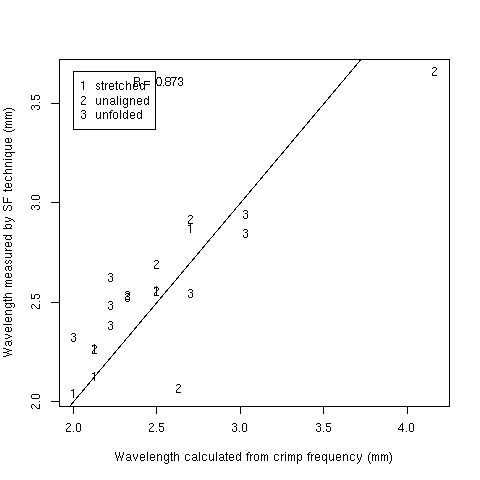
\includegraphics[width=1.0\textwidth]{figcrimpwavlsf.png}
%   crimpwavlsf.png is original 
  \caption{Correlation between wavelength calculated from staple crimp frequency and wavelength measured by the SF technique}
  \label{fig:crimpwavlsf}
\end{figure}

%\end{document}


%\documentclass{article}
%\usepackage{graphicx,subfigure}
%\begin{document}

\begin{figure}[!hb]
  \centering
  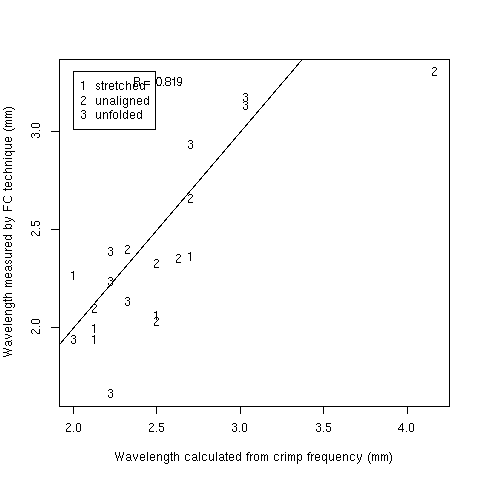
\includegraphics[width=1.0\textwidth]{figcrimpwavlfc.png}
%   crimpwavlfc.png is original 
  \caption{Correlation between wavelength calculated from staple crimp frequency and wavelength measured by the FC technique}
  \label{fig:crimpwavlfc}
\end{figure}

%\end{document}


%\documentclass{article}
%\usepackage{graphicx,subfigure}
%\begin{document}

\begin{figure}[!hb]
  \centering
  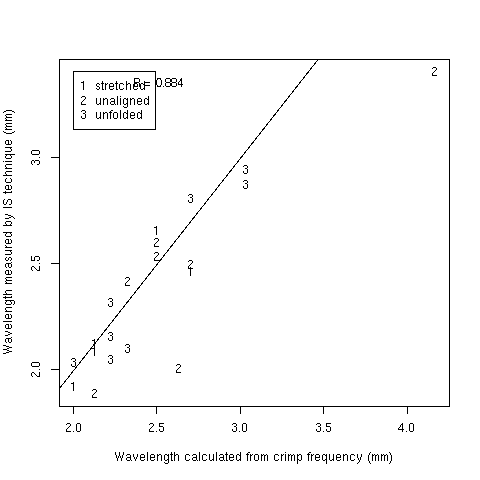
\includegraphics[width=1.0\textwidth]{figcrimpwavlis.png}
%   crimpwavlis.png is original 
  \caption{Correlation between wavelength calculated from staple crimp frequency and wavelength measured by the IS technique}
  \label{fig:crimpwavlis}
\end{figure}

%\end{document}


They are all good. Correlations greater than 0.8 and not much sign of a bias. The FC graph shows a bit more scatter, and the lowest correlation.

Figures~\ref{fig:crimpwavlsfbase}, ~\ref{fig:crimpwavlsfmid}, and ~\ref{fig:crimpwavlsftip} show the correlation with wavelength calculated from staple crimp frequency for the SF technique on the base, mid, and tip regions respectively. 
%\documentclass{article}
%\usepackage{graphicx,subfigure}
%\begin{document}

\begin{figure}[!h]
  \centering
  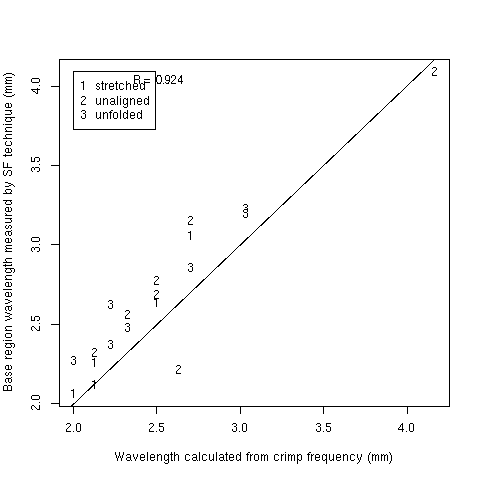
\includegraphics[width=1.0\textwidth]{figcrimpwavlsfbase.png}
%   crimpwavlsfbase.png is original 
  \caption{Correlation between wavelength calculated from staple crimp frequency and base region wavelength measured by the SF technique}
  \label{fig:crimpwavlsfbase}
\end{figure}

%\end{document}


%\documentclass{article}
%\usepackage{graphicx,subfigure}
%\begin{document}

\begin{figure}[!h]
  \centering
  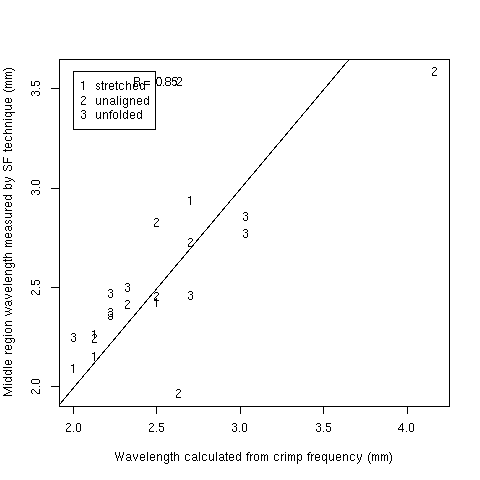
\includegraphics[width=1.0\textwidth]{figcrimpwavlsfmid.png}
%   crimpwavlsfmid.png is original 
  \caption{Correlation between wavelength calculated from staple crimp frequency and middle region wavelength measured by the SF technique}
  \label{fig:crimpwavlsfmid}
\end{figure}

%\end{document}


%\documentclass{article}
%\usepackage{graphicx,subfigure}
%\begin{document}

\begin{figure}[!h]
  \centering
  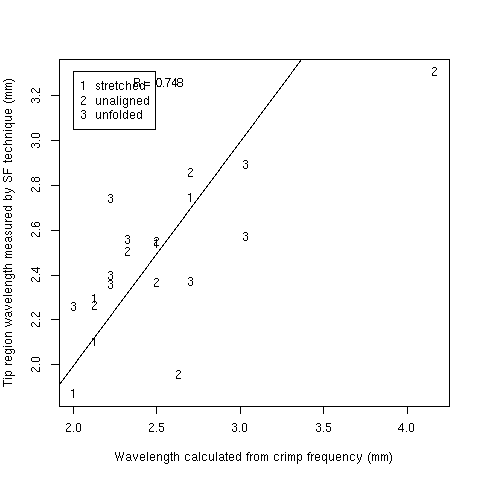
\includegraphics[width=1.0\textwidth]{figcrimpwavlsftip.png}
%   crimpwavlsftip.png is original 
  \caption{Correlation between wavelength calculated from staple crimp frequency and tip region wavelength measured by the SF technique}
  \label{fig:crimpwavlsftip}
\end{figure}

%\end{document}


They are also all well correlated, the tip region showing slightly more scatter. For the base region there is a suggestion of bias, the measured wavelength being larger than that obtained from crimp frequency by about 0.2 mm. That is not surprising because the crimp meter measures a considerable length of the staple and probably does not incluse the waves right at the base. 

If there is a bias in the base region with SF technique, there should also be a small bias in the overall SF technique. If we look back at  Figure~\ref{fig:crimpwavlsf} we can actually see that there is an excess of points above the one-to one line. 

It might be thought that having all techniques highly correlated with wavelength derived from crimp frequency conflicts with the cross-technique repeatabilities reported in Section~\ref{sec:repty}. However, remember that the repeatabilities reported in Section~\ref{sec:repty} are for the base wave only - ie the single wave at the base of the staple. The cross-technique correlations for the full set of waves at the sheep level are SF x FC r = 0.72, SF x IS r = 0.86, FC x IS r = 0.79.  These are all high.  All techniques are highly correlated with one another and all are highly correlated with wavelength derived from crimp frequency.

If we look ar the regions separately, for the SF technique, the cross-region rtepeatabilities are base x mid r = 0.94, base x tip r = 0.89, and mid x tip r = 0.92. In other words, all regions are well correlated with wavelength from crimp frequency and with each other, there is just the small bias for the base region.

If we look at each crimptype separately, the mean wavelength derived from crimp frequency is stretched 2.13 mm, unaligned 2.50 mm, and unfolded 2.27 mm. If we were to plot these means on Figures~\ref{fig:unfold}, \ref{fig:stretch}, and ~\ref{fig:unalign} they would be in line with the FC technique for stretched and unaligned wools, and slightly below the FC technique for unfolded wools. So it is clearly the SF technique which is different, and it is most different at the base end.

We have to conclude that our wavelength measurements are correct except for a small bias in the SF technique, mainly in the base region. Therefore most of the issues noted above in comparisons with OFDA must be due to problems with our amplitude measurement.  The corresponding cross-technique correlations for the full set of waves at the sheep level for amplitude measurement are SF x FC r=0.39, SF x IS r = 0.35, and FC x IS 0.91. So amplitude is quite different - SF amplitude is not highly correlated with FC or IS, but FC and IS are highly correlated with each other. 

Within the SF technique cross region repeatabilities for amplitude are base x mid r = 0.92, base x tip r = 0.75, and mid x tip r = 0.85. So SF measures amplitude repeatably, it just doesnt agree with FC or IS amplitude.

If we look back at Figures~\ref{fig:unfold}, \ref{fig:stretch}, and ~\ref{fig:unalign} only stretched and unaligned wools have an amplitude difference between SF and the other techniques, SF measuring a larger amplitude  by about 0.6 to 1.0 mm. Unfolded wools actually had SF measuring a smaller amplitude by about 0.1 mm. This interaction may be contributing to the poor correlations observed above.What it means is that something happens to the amplitude of crimp waves when a fibre is removed from a staple, and that what happens depends on whether the crimp is stretched helix or unfolded helix.  



\clearpage
\section{Assessing measurement techniques by calculating model-predictions of average fibre length}

 Using the procedure detailed in Jackson and Watts(2016)~\cite{jack:16}, we were able to calculate predictions of average fibre length  for each sheep.  Because we have actual mean fibre length measurements for each sheep, we can use this calculation to compare the SF, FC, and IS techniques for wavelength and amplitude measurement.

In the Figures showing results of prediction in the following three Sections, the lines joining the outer points of each cluster are a convex hull, and the colour-shaded area of the convex hull  is an indication of where additional data might fall. This is not a substitute for a proper statistic , the correlation denoted as $R = xxx$ provides that. The two means are given to indicate whether there is a bias in prediction. The black 45 degree line is the line on which all poinrts should fall if the prediction were perfect and the measured $Lf$ had no errors.


It can be seen from the formulae of Jackson and Watts(2016)~\cite{jack:16}, that prediction of mean fibre length involves using predicted intrinsic radius to calculate the arc-length of one crimp wave, and then  scaling this up to the arc-length of all the waves in the staple by multiplying by a quantity we call $T$ which is the number of crimp waves in a staple.

Obtaining a value for $T$ involves a number of additional assumptions over and above those involved in prediction of intrinsic radius. It requires a measure of staple length, in addition to the measures of crimp wavelength and amplitude. We must assume that all fibres extend from base to tip of the staple, so that using

\begin{equation}
\label{eqn:T}
T = L_{s}/\lambda
\end{equation}

where $L_{s}$ is staple length and $\lambda$ is wavelength,
calculates the number of waves in a staple. There is an implied assumption that this is also the number of waves in any single fibre or bundle of fibres.


So what equation~\ref{eqn:T} above for $T$ would yield, if applied to a single measured wavelength of a fibre or bundle of fibres, would be the number of crimp waves which that fibre or bundle would have, {\em if} it extended the full staple length. If the fibre or bundle did not extend to the staple tip, it would have a projected\_length shorter than the staple length, and the number of crimp waves $(T)$ would be overestimated by equation~\ref{eqn:T}. This , in turn would lead to overestimation of fibre length.

There are two options for calculating $T$

\begin{description}
\item[Method 1] convert the crimp frequency measurement for a sheep to wavelength and use that wavelength in equation~\ref{eqn:T} to calculate $T$. This provides a measure of $T$ which is independent of the fibre or bundle amplitude and wavelength measurements, and is a constant for each sheep.
\item[Method 2] use every individual wavelength measurement to calculate a $T$ for that fibre or bundle, assuming it extends the full length of the staple. Then pool the resulting predictions. This makes no attempt to allow for fibres not extending to the staple tip. This provides a measure of $T$ which varies with each wavelength measurement, but is still dependent on staple length.
\end{description}

\subsection{Model-prediction of sheep mean fibre length}
Most interest is in being able to calculate the mean fibre length for a sheep. To do this we use our model equations to calculate a predicted fibre length from the wavelength and amplitude of each individual crimp wave. We then pool these over all waves in each fibre and over all fibres to get a mean predicted fibre length for each sheep. We do the transform to fibre length first, and the pooling after, because the transform is not linear.

Results for Method 1 are shown in Figures~\ref{fig:ispredlftc} and ~\ref{fig:fcpredlftc} and ~\ref{fig:sfpredlftc}, separately for the three measurement techniques. 

%\documentclass{article}
%\usepackage{graphicx,subfigure}
%\begin{document}

\begin{figure}[!h]
  \centering
  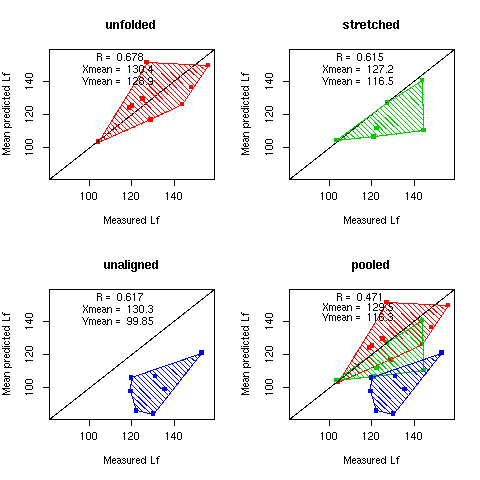
\includegraphics[width=1.1\textwidth]{figispredlftc.png}
% original is nis.5.10.predlftc.lf.png
  \caption{Plots of measured fibre length against predicted mean fibre length using Method 1 with predictions based on measurement of wavelength and amplitude by the IS technique, and crimps per staple calculated by equation ~\ref{eqn:T}. Fibre lengths for the unfolded crimp type wools were adjusted for the effect of twist at the points of inflection using $H = 0.5 * amplitude$ and $R = 0.10 mm$ in the prediction equations.}
  \label{fig:ispredlftc}
\end{figure}

%\end{document}


%\documentclass{article}
%\usepackage{graphicx,subfigure}
%\begin{document}

\begin{figure}[!h]
  \centering
  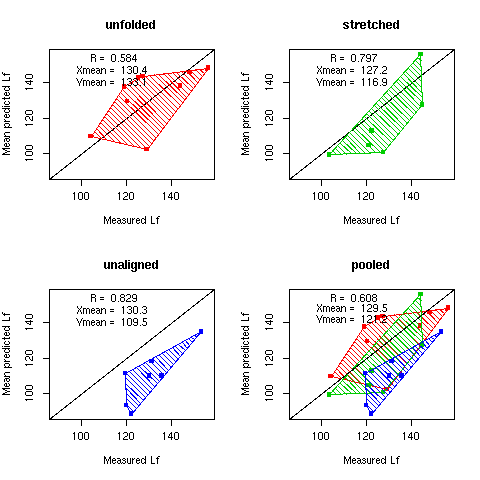
\includegraphics[width=1.1\textwidth]{figfcpredlftc.png}
% original is nfc.5.10.predlftc.lf.png
  \caption{Plots of measured fibre length against predicted mean fibre length using Method 1 with predictions based on measurement of wavelength and amplitude by the {\em fibre-mount} technique, and crimps per staple calculated by equation ~\ref{eqn:T}. Fibre lengths for the unfolded crimp type wools were adjusted for the effect of twist at the points of inflection using $H = 0.5 * amplitude$ and $R = 0.10 mm$ in equation ~\ref{eqn:lf}.}
  \label{fig:fcpredlftc}
\end{figure}

%\end{document}


%\documentclass{article}
%\usepackage{graphicx,subfigure}
%\begin{document}

\begin{figure}[!h]
  \centering
  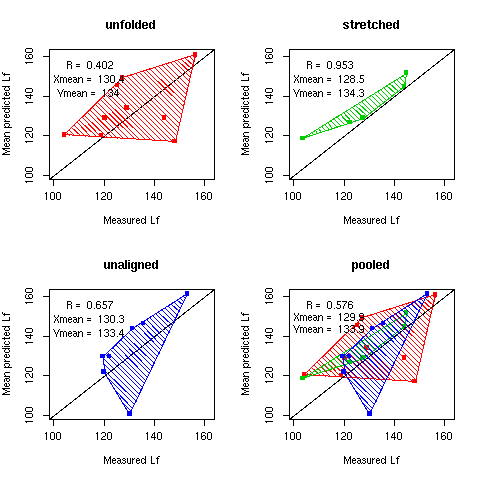
\includegraphics[width=1.1\textwidth]{figsfpredlftc.png}
% original is 21sheeppredlfmeanm1ls.png
  \caption{Plots of measured fibre length against predicted mean fibre length using Method 1 with predictions based on measurement of wavelength and amplitude by the SF technique, and crimps per staple calculated by equation ~\ref{eqn:T}. Fibre lengths for the unfolded crimp type wools were adjusted for the effect of twist at the points of inflection using $H = 0.5 * amplitude$ and $R = 0.10 mm$ in the prediction equations.}
  \label{fig:sfpredlftc}
\end{figure}

%\end{document}



There is a marked underestimation of fibre length for the {\em unaligned} wools, using measurements of wavelength and amplitude from the IS and FC techniques, but not for the SF technique.  There is also a slight underestimation for the {\em stretched} wools with the IS and SF techniques. It would seem that it is not easy to measure wavelength and amplitude properly with the fibres in the staple formation for unaligned wools, and also to a less extent for stretched wools. To measure wavelength and amplitude successfully in the staple would seem to require the very high degree of fibre alignment found only in {\em unfolded} wools. 

We think that what happens when an operator attempts to measure wavelength and amplitude either in the staple or in a multi-fibre mount, is that the operator tends to select for measurement fibres that are well aligned with their neighbours. Thus the fibres chosen for measurement would not be chosen randomly, and a bias in the measurements could result. With the SF technique fibres are chosen at random and are removed from their neighbours, so this issue does not arise.

Results for Method 2 are shown in Figures~\ref{fig:ispredlf} , ~\ref{fig:fcpredlf}, and ~\ref{fig:sfpredlf} separately for the three measurement techniques.

%\documentclass{article}
%\usepackage{graphicx,subfigure}
%\begin{document}

\begin{figure}[!h]
  \centering
  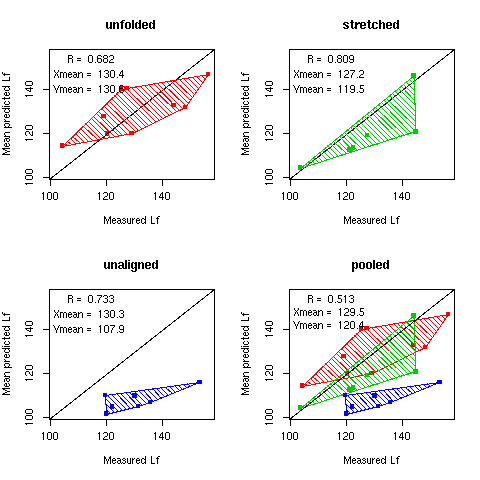
\includegraphics[width=1.1\textwidth]{figispredlf.png}
% original is nis.5.10.predlf.lf.png
  \caption{Plots of measured fibre length against predicted mean fibre length using Method 2 with predictions based on measurement of wavelength and amplitude by the IS technique, and crimps per staple calculated by equation ~\ref{eqn:T}. Fibre lengths for the unfolded crimp type wools were adjusted for the effect of twist at the points of inflection using $H = 0.5 * amplitude$ and $R = 0.10 mm$ in the prediction equations.}
  \label{fig:ispredlf}
\end{figure}

%\end{document}


%\documentclass{article}
%\usepackage{graphicx,subfigure}
%\begin{document}

\begin{figure}[!h]
  \centering
  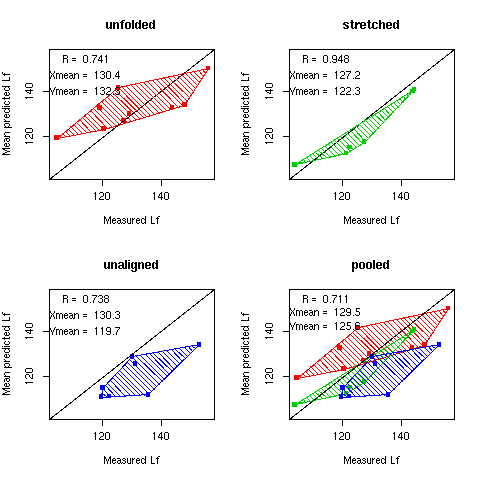
\includegraphics[width=1.1\textwidth]{figfcpredlf.png}
% original is nfc.5.10.predlf.lf.png
  \caption{Plots of measured fibre length against predicted mean fibre length using Method 2 with predictions based on measurement of wavelength and amplitude by the {\em fibre-mount} technique, and crimps per staple calculated by equation ~\ref{eqn:T}. Fibre lengths for the unfolded crimp type wools were adjusted for the effect of twist at the points of inflection using $H = 0.5 * amplitude$ and $R = 0.10 mm$ in equation ~\ref{eqn:lf}.}
  \label{fig:fcpredlf}
\end{figure}

%\end{document}


%\documentclass{article}
%\usepackage{graphicx,subfigure}
%\begin{document}

\begin{figure}[!h]
  \centering
  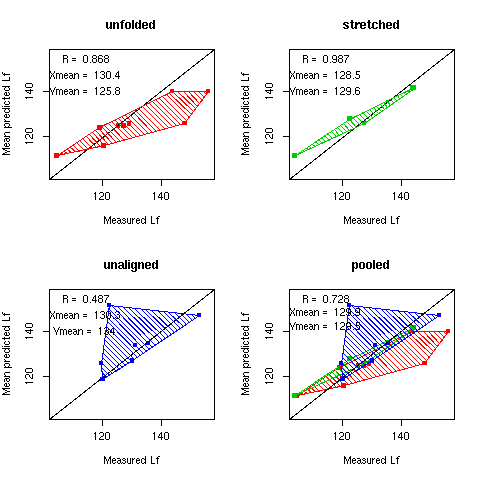
\includegraphics[width=1.1\textwidth]{figsfpredlf.png}
% original is 21sheeppredlfmeanm2ls.png
  \caption{Plots of measured fibre length against predicted mean fibre length using Method 2 with predictions based on measurement of wavelength and amplitude by the SF technique, and crimps per staple calculated by equation ~\ref{eqn:T}. Fibre lengths for the unfolded crimp type wools were adjusted for the effect of twist at the points of inflection using $H = 0.5 * amplitude$ and $R = 0.10 mm$ in the prediction equations }
  \label{fig:sfpredlf}
\end{figure}

%\end{document}



Results for Method 2 are similar to those for Method 1. The correlations within each crimp type are a little higher for Method 2 compared to Method 1. The bias is about the same for both methods. It woulld seem that either method of obtaining $T$ is satisfactory but that Method 2 is a little more accurate. There is a suggestion in the Method 2 results that the regression of predicted fibre length on measured fibre length is flatter than the one-to-one line shown on the graphs. One would need more data to be sure of this.

\subsection{Model prediction of lengths of individual fibres}
For a more accurate check on the correctness of our crimp model equations, there is interest in calculating a predicted length for each fibre. This is only possible for the SF technique where individual fibre measurements of wavelength and amplitude have been made, and where relaxed fibre length ($L_{r}$) and stretched fibre length ($L_{f}$) were also measured on the same fibre.

 To do individual fibre length predicttions, we use our model equations to calculate a predicted fibre length from the wavelength and amplitude of each individual crimp wave. We then pool these over all waves in each fibre to get a mean predicted fibre length for each fibre. We do the transform to fibre length first, and the pooling after, because the transform is not linear. In this case it is only appropriate to use Method 2 to obtain $T$, and we should modify Method 2 to use relaxed fibre length ($L_{r}$), instead of staple length ($L_{s}$), because it has been observed (Figure~\ref{fig:LrLs}) that fibres become longer than staple length on removal from the staple.

 Figure~\ref{fig:sfpredlffibre} shows the predicted lengths of 315 fibres from 21 sheep of all crimp types plotted against the measured length of the same fibre.

%\documentclass{article}
%\usepackage{graphicx,subfigure}
%\begin{document}

\begin{figure}[!h]
  \centering
  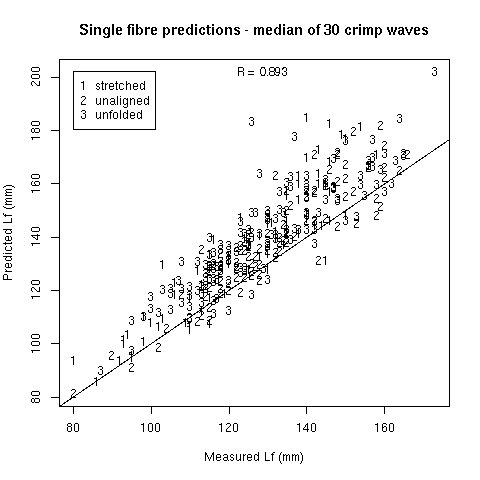
\includegraphics[width=1.1\textwidth]{figsfpredlffibre.png}
% original is 15fibrepredlfmedian.png
  \caption{Plot of measured fibre length against predicted mean fibre length for 315 individual fibres using Method 2 with predictions based on measurement of wavelength and amplitude by the SF technique, and crimps per staple calculated using relaxed fibre length instead of staple length. Fibre lengths for the unfolded crimp type wools were adjusted for the effect of twist at the points of inflection using $H = 0.5 * amplitude$ and $R = 0.10 mm$ in the prediction equations }
  \label{fig:sfpredlffibre}
\end{figure}

%\end{document}


The correlation is high and there seems to be a slight overpredict for long fibres. The two outlier points at the top of the graph are {\em unfolded} crimp type. They are more difficult to predict because the angle between unfoldings must be estimated as well as the intrinsic radius.  

 Overall, Figure~\ref{fig:sfpredlffibre} provides a convincing verification of our crimp model equations, and a demonstration that wavelength and amplitude measurements by the SF technique are correct.  

\clearpage
\section{Assessing measurement techniques by calculating model-predictions of fibre length to staple length ratio}

 Calculation of fibre length to staple length ratio from the formulae of Jackson and Watts(2016)~\cite{jack:16} is an entirely different matter to calculation of mean fibre length. Calculation of fibre length to staple length ratio does not require an estimate of $T$, the number of crimp waves in the staple. We only need the intrinsic radius calculation ( and angle between unfoldings in the case of unfolded crimp type wools), so the errors of estimating $T$ do not enter into the result. What the formulae actually calculate for each wavelength/amplitude measurement pair is the ratio of the arc-length of the measured fibre or bundle over one wave to the projected-length of one wave ( ie the wavelength). 

 Of course, if the fibre actually goes the full length of the staple, the above ratio will be the same as fibre length to staple length ratio. To show this simply multiply top and bottom of the above ratio by $T$, the number of crimp waves in a staple.

 However, if the fibre does not go right to the staple tip, what the above ratio estimates is the ratio of fibre arc-length to the projected-length of the fibre as it sits in the staple.  This will be larger than the fibre length to staple length ratio if there are some short fibres, so there may be some bias in calculations from our formulae, if the staple contains fibres which do not extend to the staple tip. This is most likely in {\em unaligned} crimp type wools.

\subsection{Model-prediction of sheep mean fibre length to staple length ratio.}
Let us do some calculations of sheep mean fibre length to staple length ratio  and see how they compare to measured fibre length to staple length ratio for each sheep. Again we do this separately for measurements of wavelength an amplitude by the IS, FC, and SF techniques. We use only Method 2 because we want the ratio of arc length to wavelength for each crimp wave, which we then pool across all waves and all fibres to get a sheep mean. The results are shown in Figures~\ref{fig:ispredlfr} , ~\ref{fig:fcpredlfr} and ~\ref{fig:sfpredlfr}.

%\documentclass{article}
%\usepackage{graphicx,subfigure}
%\begin{document}

\begin{figure}[!h]
  \centering
  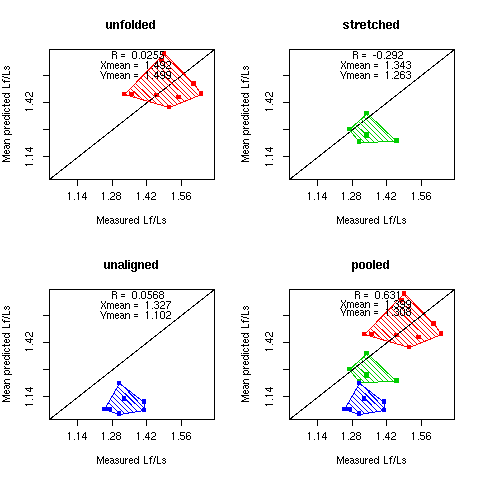
\includegraphics[width=1.1\textwidth]{figispredlfr.png}
% original is nis.5.10.predlfr.png
  \caption{Plots of measured fibre length to staple length ratio against predicted mean fibre length to staple length ratio with predictions based on measurement of wavelength and amplitude by the {\em in-staple} technique. Fibre lengths for the unfolded crimp type wools were adjusted for the effect of twist at the points of inflection using $H = 0.5 * amplitude$ and $R = 0.10 mm$ in equation ~\ref{eqn:lf}.}
  \label{fig:ispredlfr}
\end{figure}

%\end{document}


%\documentclass{article}
%\usepackage{graphicx,subfigure}
%\begin{document}

\begin{figure}[!h]
  \centering
  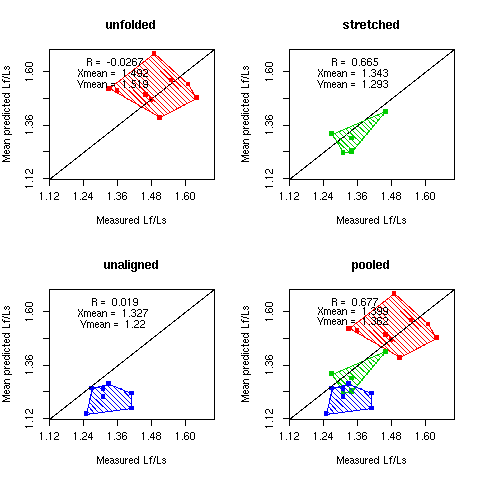
\includegraphics[width=1.1\textwidth]{figfcpredlfr.png}
% original is nfc.5.10.predlfr.png
  \caption{Plots of measured fibre length to staple length ratio against predicted mean fibre length to staple length ratio with predictions based on measurement of wavelength and amplitude by the FC technique. Fibre lengths for the unfolded crimp type wools were adjusted for the effect of twist at the points of inflection using $H = 0.5 * amplitude$ and $R = 0.10 mm$ in the prediction equations.}
  \label{fig:fcpredlfr}
\end{figure}

%\end{document}


%\documentclass{article}
%\usepackage{graphicx,subfigure}
%\begin{document}

\begin{figure}[!h]
  \centering
  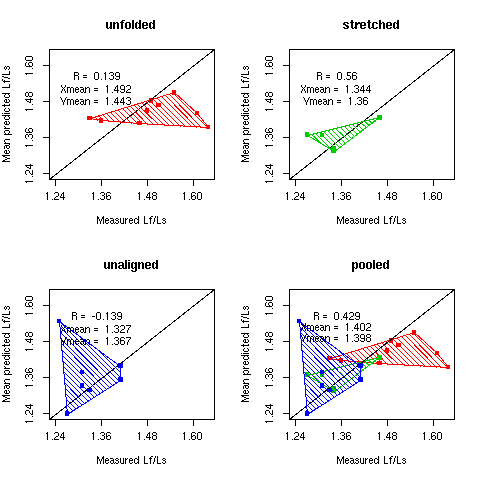
\includegraphics[width=1.1\textwidth]{figsfpredlfr.png}
% original is 21sheep15fibrepredlftolsmean.png
  \caption{Plots of measured fibre length to staple length ratio against predicted mean fibre length to staple length ratio with predictions based on measurement of wavelength and amplitude by the SF technique. Fibre lengths for the unfolded crimp type wools were adjusted for the effect of twist at the points of inflection using $H = 0.5 * amplitude$ and $R = 0.10 mm$ in the prediction equations.}
  \label{fig:sfpredlfr}
\end{figure}

%\end{document}




 There is a severe underprediction of fibre length to staple length ratio for the {\em unaligned} wools with amplitude and wavelength measued by either the IS or FC techniquea, but no bias for any of the crimptypes when wavelength and amplitude are measured by the SF technique. If there had been a problem with short fibres we expected some overprediction. This did not happen so we have to conclude that short fibres are not an issue.

The predictions of sheep mean fibre length to staple length ratio follow the same pattern as the predictions of sheep mean fibre length. The SF technique is the only one with unbiased predictions. However the correlation among sheep within each crimp type is poor. This is different from the results for prediction of mean fibre length, where the correlations among sheep within each crimp type were high. This means that for fibre length prediction variations in $T$, the number of crimps per staple are affecting the result, whereas for fibre length to staple length ratio  prediction, the result depends only on intrinsic radius. Apparently intrinsic radius has higher errors than $T$.

The result is nevertheless sufficiently good to confirm our crimp model equations.

\subsection{Model-prediction of ratio of stretched length to relaxed length of individual fibres.}
We may get a more accurate check of our crimp model equations if we calculate a predicted ratio of relaxed length to stretched length for each fibre. This is only possible for the SF technique.

To do indivdual fibre predictions we simply pool our predicted ratio of arc length to wavelength across all waves in a fibre, but not across fibres. 

Figure~\ref{fig:predlftolrfibre} shows the predicted fibre stretched length to fibre relaxed length ratio, plotted against measured stretched length to relaxed length ratio for 315 fibres from 21 sheep of all crimp types. 

%\documentclass{article}
%\usepackage{graphicx,subfigure}
%\begin{document}

\begin{figure}[!h]
  \centering
  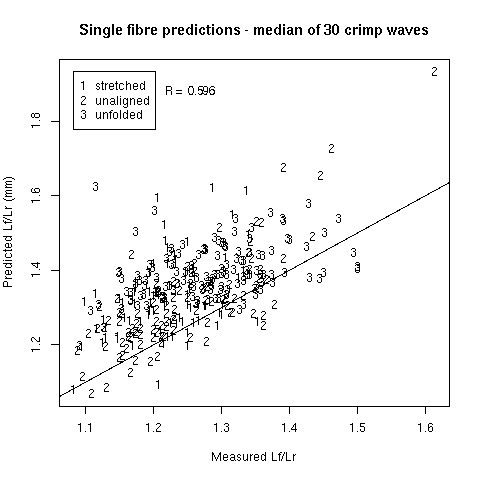
\includegraphics[width=1.1\textwidth]{figpredlftolrfibre.png}
% original is 15fibrepredlftolrmedian.png
  \caption{Plot of measured fibre stretched length to relaxed length ratio against predicted mean fibre stretched length to relaxed length ratio for 315 individual fibres with predictions based on measurement of wavelength and amplitude by the SF technique, and the ratio calculated using relaxed fibre length instead of staple length. Fibre lengths for the unfolded crimp type wools were adjusted for the effect of twist at the points of inflection using $H = 0.5 * amplitude$ and $R = 0.10 mm$ in the prediction equations }
  \label{fig:predlftolrfibre}
\end{figure}

%\end{document}



Because the measured relaxed and stretched lengths are on the same fibre as the wavelength and amplitude measurements, we get a better correlation of predicted with measured ratio here. There is, however, a small bias. The ratio is overpredicted by about 0.1 units. There is no sign of any particular crimptype being involved in this bias. They are just all a fraction too large. 

Remember that fibre length prediction for individual fibres was similaraly biased. The phenomenon may be related to the changes in wavelength and amplitude along the fibre observed in Figures~\ref{fig:unfold}, \ref{fig:stretch}, and ~\ref{fig:unalign}.

Note that these single fibre predictions  of $L_{f}/L_{r}$ are not a prediction of fibre length to staple length ratio ($L_{f}/L_{s}$). We can see this by plotting these two ratios using actual measurements, not predictions. This plot is shown in Figure~\ref{fig:fibrelftolslftolr}.
%\documentclass{article}
%\usepackage{graphicx,subfigure}
%\begin{document}

\begin{figure}[!h]
  \centering
  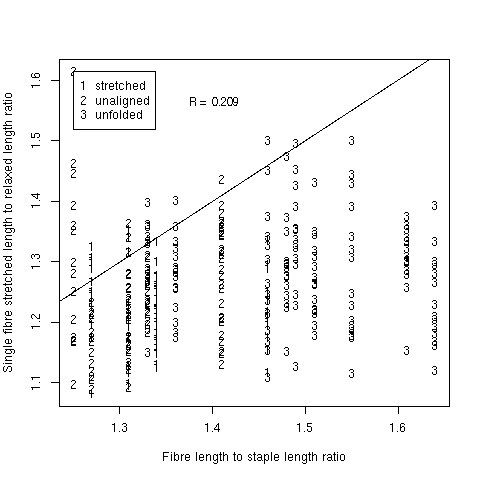
\includegraphics[width=1.1\textwidth]{figfibrelftolslftolr.png}
% original is  15fibrepredLftoLrmedian.png
  \caption{Plot of measured fibre stretched length to relaxed length ratio for 15 fibres per sheep, against measured mean fibre stretched length to staple length ratio for each sheep. }
  \label{fig:fibrelftolslftolr}
\end{figure}

%\end{document}


We see that there is practically no relationship and that $L_{f}/L_{r}$ is smaller than the corresponding $L_{f}/L_{s}$. That is because $L_{r}$ is longer than $L_{s}$. We defer an explanation of this phenomenon to the next section.

The software used to make the above predictions is available in Appendix A.

\clearpage
\section{Explanation of the results obtained from our various assessments of wavelength and amplitude measurement techniques}

We have collected a large number of facts based on careful measurement and comprehensive analysis. It is time to see if we can draw these together into a consistent explanation of crimp formation which enables us to see why particular ways of observing wavelength and amplitude lead to particular results.

The crimp model developed by Jackson and Watts (2016)~\cite{jack:16} says that fibres grow from the follicles with an intrinsic curvature or radius forming a helix which is either stretched or unfolded, as the fibre grows, and is 'set' in that position, and stays that way as the staple grows longer, simply moving up as the fibres continue to grow below it. 

So, according to the Jackson and Watts (2016)~\cite{jack:16} model, if we measure wavelength and amplitude of fibres anywhere along the staple, we should be able to use our model equations to back-calculate from observed wavelength and amplitude to intrinsic radius, and from there to fibre length and fibre length to staple length ratio. But, it doesnt work. We underpredict fibre length for unaligned and stretched helix wools. There is also a bias in comparison with OFDA mean curvature for unaligned and stretched wools.

Why? Because something else happens to the fibres in the staple , after the initial stretch or unfold is 'set'. The 'set' crimp waves are compressed - ie the projected fibre length (= staple length) becomes slightly shorter, and each of the waves is reduced in wavelength.

What force is responsible for this compression? Possible forces are 
\begin{itemize}
\item the growing mass of fibres push up on the 'set' crimp waves above them
\item the fibre scales cause a 'felting-like' phenomenon, aided by movement of the sheep, which tends to push the fibres towards the staple base. Because the base is anchored in the follicle, the whole fibre cannot move as in felting, so it compresses, reducing the wavelengths and increasing the amplitudes.
\item some external force, as when belly wool rests on the ground.
\end{itemize}

We favour the second of these hypotheses.

What this secondary movement phenomenon does is take our fibre wavelengths and amplitudes out of the stretched or unfolded helix position which is described by our crimp model.

Therefore, if we measure wavelength and amplitude in the staple ( FC or IS technique) we cannot successfully back-calculate to intrinsic radius from these wavelengths and amplitudes, so our predictors of fibre length and fibre length to staple length ratio will fail. There will be a bias, and we have observed one.

What we need to do is remove fibres from the staple, let them relax back into the position of their 'crimp set', measure wavelength and amplitude in this relaxed position, and then do our prediction of fibre length and fibre length to staple length ratio. This is what the SF technique does, and it works. There is no bias using wavelengths and amplitudes from the SF technique.


Why do the fibres relax back to a longer length than the staple? Because the positions the fibres take up in the staple under the compression force are not 'set' like the stretched or unfolded helix is 'set'. They are held in a compressed position under tension by contacts with the surrounding fibres. We have used the term 'handcuffed' to describe fibres held in this state of tension.

Why are the fibres not set in the compressed position?. Because the conditions for setting ( heat and moisture) are probably only present near the skin surface, where the stretching and unfolding occur. Also the compression process is probably continuous. So when each fibre is 'released' from its staple ( handcuffs removed), the tensions caused by the compression are able to relax out, and the fibre gets longer and each wavelength increases.  So relaxed fibre length can be seen as what the staple length would have been if there had been no compression.

Why are wavelengths greater at the base of a relaxed fibre? We dont know. Possibilities are
\begin{itemize}
\item a phenomenon peculiar to this flock ( we only have data on one flock)
\item less compression at the staple base, or conversely more compression at the staple tip. This seems likely. If the compression process is continuous the tip ends of fibres would undergo it for longer.
\item more relaxation at the staple base after fibre removed from staple
\item less relaxation at the staple tip after fibre removed from staple
\end{itemize}


We favour the second of these. 

The case of unfolded wools requires some more thought. They do not underpredict if we use in-staple (IS or FC) measures of wavelength and amplitude, and they are also unbiased with the SF technique. So we need to think about what happens to an unfolded helix if it is compressed. 

Under compression, an unfolded helix does not behave like a spring. It either can 'concertina' in one plane, or it can bend out of the plane and become a 3D object - a dished semicircular wave.We do not know which of these happens in practice. but in either case there will be bends under tension, and these will relax out when the fibre is taken from the staple. So the fibre should elongate just like the stretched helix wools, and this is what we observe.

However, the interpretaton of wavelength and amplitude differs. If we consider the 'concertina' option, the reason in-staple (IS or FC) technique leads to unbiased prediction from wavelength and amplitude for unfolded wools, is that our crimp model for unfolding actually allows for the 'concertina' effect by computing angle between unfoldings ($\theta$) as well as intrinsic radius. When a fibre with unfolded helix crimp is 'concertinad' it attains
\begin{itemize}
\item lower wavelength
\item slightly larger amplitude
\item larger $\theta$ ( more horseshoe shape)
\item smaller radius ( tighter curves)
\end{itemize}
Then, when the fibre is relaxed, it simply returns to the lower $\theta$ and larger radius shape. Our model for unfolded crimp can compute  the fibre length correctly from either the compressed wavelength and amplitude in the staple, or from the relaxed wavelength and amplitude in the removed fibre. It can do this because it uses $\theta$ as well as radius, and $\theta$ serves as an index of amount of concertina. It would not however compute intrinsic radius correctly from in-staple measurements of wavelength and amplitude, because it assumes that the radius that it sees {\em is} the intrinsic radius. This does not affect fibre length calculation because we can get fibre length from any radius provided it is accompanied by a matching $\theta$.

This lines up with what we have observed for unfolded helix wools in Figure~\ref{fig:unfold}. In the staple the unfolded wools have lower wavelengths and slightly larger amplitudes compared to in the removed fibre.

We can check further by comparing $\theta$ and intrinsic radius estimates based on the three techniques. These are shown in Table~\ref{tab:concertina} for each of the eight sheep with unfolded wool. 
% latex table generated in R 3.2.4 by xtable 1.8-2 package
% Sat Sep 17 20:21:29 2016
\begin{landscape}
\begin{table}[ht]
\centering
\caption{Measured wavelength and amplitude together with calculated intrinsic radius and $\theta$ for eight sheep with unfolded crimp type. The SF measurements and calculated values are on single fibres removed from the staple and relaxed, the FC and IS measurements and calculated values are on fibre crimp waves in the staple. The staple length ($L_{s}$) and relaxed fibre length ($L_{r}$)  and their ratio ($L_{s}/L_{r}$) are presented to show that all eight sheep had staples which had contracted to less than the relaxed fibre length}
\label{tab:concertina}
\begin{tabular}{p{0.3in}|p{0.3in}|p{0.3in}|p{0.3in}|p{0.3in}|p{0.3in}|p{0.3in}|p{0.3in}|p{0.3in}|p{0.3in}|p{0.3in}|p{0.3in}|p{0.3in}|p{0.3in}|p{0.3in}|p{0.3in}}
  \hline
  Sheep No & SF Wavelength & SF Amplitude & SF Intrinsic Radius & SF $\theta$ & FC Wavelength & FC Amplitude & FC Intrinsic Radius & FC $\theta$ & IS Wavelength & IS Amplitude & IS Intrinsic Radius & IS $\theta$ & $L_{s}$ & $L_{r}$ & $L_{s}/L_{r}$ \\ 
  \hline
  1  & 2.32 & 0.36 & 0.65 & 126.7 & 1.94 & 0.38 & 0.50 & 152.2 & 2.03 & 0.38 & 0.53 & 146.6 & 97.1 & 115.6 & 0.84 \\ 
  2  & 2.52 & 0.41 & 0.69 & 131.1 & 2.13 & 0.41 & 0.55 & 149.8 & 2.10 & 0.35 & 0.57 & 135.6 & 78.4 & 85.0 & 0.92 \\ 
  3  & 2.62 & 0.46 & 0.70 & 140.3 & 2.23 & 0.55 & 0.56 & 177.9 & 2.05 & 0.48 & 0.51 & 172.4 & 84.0 & 98.9 & 0.85 \\ 
  4  & 2.84 & 0.48 & 0.76 & 136.9 & 3.13 & 0.48 & 0.87 & 127.0 & 2.87 & 0.49 & 0.77 & 136.9 & 95.3 & 116.4 & 0.82 \\ 
  5  & 2.94 & 0.50 & 0.79 & 136.9 & 3.17 & 0.67 & 0.80 & 161.2 & 2.94 & 0.56 & 0.76 & 150.1 & 87.5 & 102.0 & 0.86 \\ 
  6  & 2.54 & 0.35 & 0.74 & 116.8 & 2.93 & 0.56 & 0.76 & 150.1 & 2.81 & 0.53 & 0.73 & 147.4 & 90.3 & 102.8 & 0.88 \\ 
  7  & 2.38 & 0.44 & 0.62 & 145.7 & 1.66 & 0.30 & 0.43 & 145.1 & 2.16 & 0.36 & 0.58 & 134.0 & 83.2 & 95.8 & 0.87 \\ 
  8  & 2.48 & 0.37 & 0.70 & 123.8 & 2.39 & 0.40 & 0.64 & 135.9 & 2.31 & 0.41 & 0.61 & 141.0 & 82.4 & 87.0 & 0.95 \\ 
   \hline
\end{tabular}
\end{table}
\end{landscape}

We see that the relaxed fibres ( from SF technique) have a lower $\theta$ and a larger intrinsic radius, except for sheep number 4. Sometimes looking at raw data is the best way to see what is happening. Note also that all 8 sheep have a relaxed fibre length longer than the staple length, so they all were held under tension and relaxed out to a longer length when freed from the staple. The ratio ($L_{s}/L_{r}$) does not vary a great amount between sheep, showing that all sheep had staples contracted in length by a similar amount.  This confirms our 'concertina' hypothesis for unfolded wools. Any of these calculated combinations of $\theta$ and radius will predict fibre length properly, but only the SF technique will estimate intrinsic radius correctly for unfolded wools.

We currently have no means of modelling the amount of 'compression'  or 'concertina' in staples, because we do not fully understand the forces involved. If we could do that, we could use the simpler in-staple measures of wavelength and amplitude. The idea that one could simply inspect staples visually and assess the fibre crimp correctly, has not quite been achieved, because a staple turns out to be a more complicated entity than our crimp models envisaged. Further work is required to understand how the secondary modification of crimp occurs, and to build it into a better staple crimp model.


\section{Conclusions from our various assessments of wavelength and amplitude measurement techniques}
 The original aim of investigating ways of measuring wavelength and amplitude of crimp waves was to find a means of validating prediction equations arising out of our crimp model. We have the answer to that. For the moment we have to use the SF technique for validation.

Along the way we have discovered why the SF technique is needed.  We have found that crimp is modified in the staple, after it is formed and set. We do not fully understand this phenomenon,but it probably involves a felting-like process whereby fibres ratchet toward the staple base and thereby reduce the crimp wavelength. Our current crimp model does not cover this secondary crimp modification effect, and that is why the SF technique must be used for its validation.

Our attempt to use OFDA curvature measurement as a criterion for assessing our wavelength and amplitude measurements led to some enormous complications and a mystery result. We did a least get from it an indication that the SF technique is least biased, at least for stretched helix wools. We also got some understanding of what the OFDA curvature measurement on staple preparations is, and an indication that it means something different for stretched and unfolded wools.

The statistical analysis yielded important estimates of variance components and correlations which summarize the basic variance and covariance  properties of wavelength and amplitude data. 




\begin{thebibliography}{99}

\bibitem{jack:16}
Jackson, N. and Watts, J.E. (2016) Staple crimp formation in the fleece of Merino sheep. Report available from the authors as a pdf document.

\bibitem{ofda:16}
I need an OFDA reference.

\end{thebibliography}


\appendix
\section{Appendix}
The software used to do the calculations presented in this document is available below. It consists of a set of functions written in the R statistical language and is available as free software under the GPL2 licence.

\begin{verbatim}

function(lambda,ampl,twistlen,twistrad,stalen,t){
# unfoldt() - radius of curvature, angle between unfoldings,
#	     bundle length, fibre length, and Lf/Ls ratio
#                 from wavelength (lambda) 
#		       amplitude (ampl)
#		       twistlen (length of twisted region)
#		       twistrad (radius of curvature of twist)
#		       stalen (staple length)
#                      t = crimps per staple - supplied by call
#                 for unfolded helix
  a <- iradius(lambda,ampl)
  if(a <= 0) {
    stop(" Radius not positive in unfold()(:\n")
  }
  if(a == ampl){
    theta <- c(0,0)
    theta[2] <- 180
    theta[1] <- pi
  }
  else if( ampl < a) {
    theta <- unfanlt180(a,lambda)
  }
  else if( ampl > a) {
    theta <- unfangt180(a,lambda)
  }
    lb <- 2 * a * t * theta[1]
    lbtols <- lb/stalen
    lf <- (2 * a * theta[1] - 2 * twistlen +
                          2 * sqrt((twistlen)^2 + (pi * twistrad)^2)) * t
    lftols <- lf/stalen

  retobj <- list(radius=a,unfang=theta,t=t,lb=lb,lbtols=lbtols,lf=lf,lftols=lftols)
  return(retobj)
}
function(lambda,ampl,stalen,t)
# stretcht() - intrinsic radius of curvature, fibre length, and Lf/Ls ratio 
#             from wavelength (lambda) 
#		   amplitude (ampl)
#                  stalen (staple length)
#		   t = crimps per staple supplied by call
#             for a stretched helix
{
  as <- ampl
  bs <- lambda/(2 * pi)
  ac <- sqrt(as^2 + bs^2)
  lf <- 2 * pi * t * sqrt(as^2 + bs^2)
  lftols <- lf/stalen
  retobj <- list(radius=ac,t=t,lf=lf,lftols=lftols)
  return(retobj)
}
function(a,lambda){
#  unfangt180()  - unfolding angle in radians and degrees for theta>180
  theta <- c(0,0)
  theta[1] <- 2*(pi - asin(lambda/(4 * a)))
  theta[2] <- theta[1] * 360 / (2 * pi)
  return(theta)
}
function(a,lambda){
#  unfanlt180()  - unfolding angle in radians and degrees for theta < 180
  theta <- c(0,0)
  theta[1] <- 2 * asin(lambda/(4 * a))
  theta[2] <- theta[1] * 360 / (2 * pi)
  return(theta)
}
function(lambda,h){
# iradius() - intrinsic radius of fibre curvature
#             from wavelength (lambda) and amplitude (h)
#             for unfolded helix crimp only
  a <- (lambda^2 + 16*h^2)/(32 * h)
  return(a)
}
\end{verbatim}

The above functions are designed to process one set of values. If one wishes to do calculations for a whole table of values, and to handle a mixture of crimp types (unaligned, stretched, or unfolded) one needs to set up a calling routine which loops as follows. This function returns a 'list' object containing the individual predictions for each pair of wavelength/amplitude measurements, and the mean prediction for each sheep.

\begin{verbatim}

function(lambda,ampl,type,stalen,crimpfreq=NULL,twistlen=0.5,twistrad=0.10)
# pred()  - predict  intrinsic radius,fibre length, and Lf/Ls ratio
#           for all crimp types
#           for a matrix of values of wavelength (lambda) - nsheep x nmeas
#           and matrix of amplitudes (ampl) - nsheep x nmeas
#           crimp type (type) vector of values for each sheep
#           staple length (stalen) vector of values in mm for each sheep
#           crimpfreq - NULL or vector of values for each sheep
#	    crimpfreq - if not NULL crimpfreq is used to calculate T
#                     - if NULL T is calculated from lambda values
#	    twistlen is a constant multiplier of amplitude 
#           twistrad is a constant - twisted bundle radius in mm
{
  outlist <- vector("list",20)
  nsheep <- nrow(lambda)
  nmeas <- ncol(lambda)
  radius <- matrix(0,nsheep,nmeas)
  unfangrad <- matrix(0,nsheep,nmeas)
  unfangdeg <- matrix(0,nsheep,nmeas)
  lf <- matrix(0,nsheep,nmeas)
  lftols <- matrix(0,nsheep,nmeas)
  lb <- matrix(0,nsheep,nmeas)
  lbtols <- matrix(0,nsheep,nmeas)

# do all individual measurement predictions
  for(i in 1:nsheep){
    if(type[i] == "unfolded") {
      for(j in 1:nmeas){
        if(is.null(crimpfreq)){
          tmp <- unfoldt(lambda[i,j],ampl[i,j],ampl[i,j]*twistlen,
                  twistrad,stalen[i],stalen[i]/lambda[i,j])
        }
        else{
          tmp <- unfoldt(lambda[i,j],ampl[i,j],ampl[i,j]*twistlen,
                  twistrad,stalen[i],stalen[i] * crimpfreq[i] / 10)
        }
        radius[i,j] <- tmp$radius
        unfangrad[i,j] <- tmp$unfang[1]
        unfangdeg[i,j] <- tmp$unfang[2]
        lf[i,j] <- tmp$lf
        lftols[i,j] <- tmp$lftols
        lb[i,j] <- tmp$lb
        lbtols[i,j] <- tmp$lbtols
      }  #  end j
    }
    else if (type[i] == "stretched") {
      for(j in 1:nmeas){
        if(is.null(crimpfreq)){
          tmp <- stretcht(lambda[i,j],ampl[i,j],stalen[i],
                   stalen[i]/lambda[i,j])
        }
        else {
          tmp <- stretcht(lambda[i,j],ampl[i,j],stalen[i],
                   stalen[i] * crimpfreq[i] / 10)
        }
        radius[i,j] <- tmp$radius
        unfangrad[i,j] <- NA
        unfangdeg[i,j] <- NA
        lf[i,j] <- tmp$lf
        lftols[i,j] <- tmp$lftols
        lb[i,j] <- NA
        lbtols[i,j] <- NA
      }  # end j
    }
    else if (type[i] == "unaligned") {
      for(j in 1:nmeas){
        if(is.null(crimpfreq)){
          tmp <- stretcht(lambda[i,j],ampl[i,j],stalen[i],
                   stalen[i]/lambda[i,j])
        }
        else {
          tmp <- stretcht(lambda[i,j],ampl[i,j],stalen[i],
                   stalen[i] * crimpfreq[i] / 10)
        }
        radius[i,j] <- tmp$radius
        unfangrad[i,j] <- NA
        unfangdeg[i,j] <- NA
        lf[i,j] <- tmp$lf
        lftols[i,j] <- tmp$lftols
        lb[i,j] <- NA
        lbtols[i,j] <- NA
      }  # end j
    }
    else {
      stop("Invalid crimp type \n")
    }
  }  # end i

# average the individual measurement predictions
  for(i in 1:nsheep){
    meanradius <- apply(radius,1,mean)
    meanunfangrad <- apply(unfangrad,1,mean)
    meanunfangdeg <- apply(unfangdeg,1,mean)
    meanlf <- apply(lf,1,mean)
    meanlftols <- apply(lftols,1,mean)
    meanlb <- apply(lb,1,mean)
    meanlbtols <- apply(lbtols,1,mean)
  }  # end i

# setup outlist
   outlist <- list(Radius=radius,Unfangrad=unfangrad,Unfangdeg=unfangdeg,Lf=lf,LftoLs=lftols,Lb=lb,LbtoLs=lbtols,MeanRadius=meanradius,MeanUnfangrad=meanunfangrad,MeanUnfangdeg=meanunfangdeg,MeanLf=meanlf,MeanLftoLs=meanlftols,MeanLb=meanlb,MeanLbtoLs=meanlbtols,Lambda=lambda,Ampl=ampl,CrimpType=type,Stalen=stalen,Twistlen=twistlen,Twistrad=twistrad)
  return(outlist)
}
\end{verbatim}

\end{document}
